\chapter{Огляд методів та архітектур моделей штучного інтелекту для обробки математичних задач}

Одним з напрямків обробки природної мови є робота з математичними текстами – задачами, які можуть бути розв'язані за допомогою різноманітних методів, включаючи класифікаційні алгоритми, глибоке навчання та системи пошуку доведень. Класифікація та вивчення різних типів таких задач, а також аналіз методів до їх розв'язання, є необхідними для ефективного пошуку відповідних систем та вдосконалення механізмів розпізнавання умов задач.

У загальному вигляді математичні текстові задачі (Mathematical Text Problems, MWP) -- це задачі, які представлені природною мовою та вимагають математичного міркування для розв'язання. Зазвичай дані задачі подаються у вигляді тексту або разом з додаткового зображення. Вони є важливим інструментом для оцінки розуміння математичних можливостей систем, а також мають практичне значення у реальних ситуаціях.

Особливість розробки ефективних систем пошуку доведень полягає у тому, щоб обробити текст задач та коректно ідентифікувати важливі елементи інформації задля того, щоб продемонструвати логічну послідовність та точність у висновках.

\section{Різновиди математичних задач}

Перед тим як перейти до огляду методів роботи з математичними текстами задач опишемо деякі типи задач та їхні особливості.

Математичні текстові задачі (MWP) є поширеним типом задач, які використовуються при розробці систем автоматичного пошуку розв'язань. Класифікувати задачі можна за форматом (задачі з варіантами відповіді, розгорнуті розв'язання, короткий розв'язок тощо) або за математичними розділами (наприклад, геометрія, алгебра, комбінаторика тощо):

\begin{itemize}
    \item Задачі типу Multiple Choice (MCQ-type Questions)
    \item Алгебраїчні задачі (Algebra Problems)
    \item Геометричні задачі (Geometric Problems)
    \item Задачі на теорію чисел (Number Theory problems)
    \item Комбінаторні задачі (Mathematical Combinatorial Problems)
\end{itemize}

Окрім інших типів задач, які не наведені вище, слід зазначити, що деякі математичні задачі можуть мати властивості відразу кількох тем, наприклад, так звані комбі-геометричні задачі -- задачі, які задані у просторі певної розмірності, але передбачають певний комбінаторний підхід до їх розв'язання. Наведемо більш детальний опис відповідних типів задач.

\paragraph{Задачі з вибором кількох варіантів відповідей}
Розв'язання задач цього типу починається з аналізу текстової умови, що дозволяє ідентифікувати ключові математичні об'єкти та логічні зв'язки, присутні в задачі. Система виконує генерацію або вибір з попередньо визначеного набору можливих відповідей, після чого проводиться ретельна оцінка кожного варіанту. Використання класифікаторів або експертних правил дозволяє обрати правильну відповідь, спираючись на порівняння виділених характеристик умови з можливими відповідями. Таким чином, основна задача полягає у побудові моделі, здатної на основі вхідного тексту оцінити релевантність кожного варіанту. Здебільшого даний тип задач не є складним, адже надає обмежену кількість варіантів (зазвичай від 4 до 10) до вибору відповідей системою.  Задачі даного типу досліджуються як окремий тип за рахунок формату поданих умов, але можуть включати різні тематики (геометрія, алгебра і тд.).

\paragraph{Алгебраїчні задачі}
Алгебраїчні задачі є важливою категорією, оскільки вони вимагають трансформації текстового опису у відповідні математичні вирази та рівняння, що відображають логічну структуру задачі. До цієї категорії належать, зокрема, арифметичні словесні задачі та задачі зі системами рівнянь. Дані підтипи є найбільш активно досліджуваними завдяки їх відносній структурованості та ясності математичного моделювання, що дозволяє застосувати як символьні, так і чисельні методи розв'язання.

У розв'язанні \textbf{арифметичних словесних задач} важливо перетворити текстовий опис у математичну модель. Спочатку проводиться автоматичне відокремлення числових параметрів, операцій та невідомих, що містяться в умові. Далі формується відповідне алгебраїчне рівняння або система рівнянь, що відображає логічну структуру задачі. Для отримання точного розв'язання застосовуються як символьні, так і чисельні методи обчислення, що дозволяє перевірити коректність отриманого результату. Такий підхід об'єднує в собі можливості NLP для аналізу тексту та традиційні методи розв'язання рівнянь.

Даний тип задач характеризуються тим, що за допомогою даних текстових умов необхідно скласти відповідне рівняння та отримати відповідь на задачу. Такі задачі задаються послідовністю слів $\langle w_0, w_1, \dots, w_k \rangle$, де деякі слова є кількостями $q_0, q_1, \dots, q_n$, згаданими в тексті, а також невідомою змінною $x$. Основною метою є подання текстової задачі у вигляді відповідного рівняння $E$, яке є лінійним у даному випадку. Серед основних арифметичних операцій використовуються лише $+$, $-$, $\times$, $\div$. Арифметичні задачі були одними з перших, які досліджувалися у даній галузі за рахунок простоти у перевірці коректності складених рівнянь.

\begin{figure}[h]
    \centering
    \small
    \captionof{table}{Приклад арифметичної словесної задачі. Кольором виділені елементи задачі, які мають інформаційну цінність до запитання або є зайвими.}
    \label{tab:mwp_example}
    \begin{tabular}{|p{0.38\linewidth}|p{0.31\linewidth}|p{0.13\linewidth}|}
        \hline
        \textbf{Умова задачі} & \textbf{Рівняння до умови задачі} & \textbf{Числова відповідь} \\
        \hline
        Міша знайшов \hlgreen{35 мушель} та \hlred{7 морських зірок} на пляжі. Він віддав \hlgreen{22 мушлі} Каті. Скільки мушлей тепер має Міша? & \[ x = 35 - 22 \] & \[ 13 \] \\
        \hline
    \end{tabular}
\end{figure}

Задачі, що включають \textbf{системи рівнянь}, вимагають виділення декількох пов'язаних умов, кожна з яких може бути формалізована як окреме рівняння. Після цього будується система рівнянь, яка описує взаємозв'язок між невідомими величинами. Розв'язання таких систем може здійснюватися як символьними методами (наприклад, методом Гауса), так і чисельними алгоритмами, що дозволяє адаптувати модель до конкретних вимог задачі. Важливим аспектом є точність математичного моделювання та правильне перетворення семантичної інформації тексту у математичну форму. Дані задачі активно використовуються у задачах оптимізації.

\paragraph{Геометричні задачі}
Геометричні задачі орієнтовані на просторове мислення та вимагають особливого підходу до інтерпретації описаних у задачі геометричних об'єктів. Спершу здійснюється розпізнавання опису геометричних фігур, відрізків, кутів або інших просторових характеристик. На основі цього формується математична модель, що може містити геометричні формули для обчислення довжини, площі або об'єму. У деяких випадках задача може вимагати інтеграції з візуальними методами обробки даних, якщо поряд із текстом подається схематичне зображення. Таким чином, застосовуються як класичні геометричні алгоритми, так і сучасні методи глибокого навчання для аналізу просторових описів.

\paragraph{Задачі з теорії чисел}
Задачі з теорії чисел охоплюють широкий спектр задач, що досліджують властивості цілих чисел, такі як простота, дільники, залишки та інші властивості чисел. Розв'язання таких задач зазвичай вимагає застосування спеціалізованих теорем та алгоритмів, спрямованих на аналіз властивостей чисел. Система, яка обробляє подібні задачі, повинна мати можливість розпізнавати ключові поняття, трансформувати текстовий опис у формалізовану модель та застосовувати як символьні методи доказу, так і чисельні алгоритми для перевірки результатів. Активно досліджуваними аспектами є алгоритми щодо перевірки простоти чисел, обчислення найбільшого спільного дільника, а також застосування евристичних методів.

\paragraph{Комбінаторні задачі}
До цієї категорії відносяться задачі, які не підпадають безпосередньо під попередні типи розв'язання. Вони можуть вимагати комплексного підходу, який об'єднує декілька математичних та алгоритмічних методів для побудови адекватної моделі задачі. При розв'язанні таких задач особливо значущим є здатність моделей до відокремлення семантичної складової задачі задля пошуку необхідних теорем чи термінів, які нададуть можливість перевести задачу у формально-математичному вигляді. У деяких випадках поєднується символьний аналіз із моделями глибокого навчання для точного визначення послідовності логічних кроків. Інтеграція результатів різних методів забезпечує підвищення цієї загальної точності та дозволяє розв'язати складні задачі, що містять неоднозначності або вимагають комплексного аналізу.

Комбінаторні задачі добре підходять для оцінки математичних можливостей моделей штучного інтелекту та систем автоматичного пошуку доведень, оскільки правильні відповіді зазвичай виражені як комбінаторні формули або у звичайному числовому вигляді, що робить процес перевірки відповіді ефективним та відтворюваним. Формулювання відповідей на комбінаторні задачі може включати біноми, факторіали та інші комбінаторні символьні представлення, які також приймаються в експерименті. Приклад комбінаторної задачі з відповіддю в обох формах наведено в Таблиці~\ref{table:puzzle_example}.

\begin{figure} \centering \small
    \captionof{table}{Приклад комбінаторної задачі з відповіддю.}
    \label{table:puzzle_example}
    \begin{tabular}{|p{0.38\linewidth}|p{0.31\linewidth}|p{0.13\linewidth}|}
        \hline
        \textbf{Умова задачі} & \textbf{Комбінаторна відповідь} & \textbf{Числова відповідь} \\
        \hline
        Ліа має 2 яблука, 3 банани і 2 апельсини. Наступного тижня вона хоче з'їсти по одному фрукту кожного дня. Скільки існує способів це зробити? & \[ P(2,3,2) = \frac{7!}{2!3!2!} \] & \[ 210 \] \\
        \hline
    \end{tabular}

\end{figure}

Крім того, при наданні відповіді у вигляді комбінаторної формули зазвичай можливо витягти кроки міркування, які призвели до фінальної відповіді. Також існує можливість знайти комбінаторні задачі з широким діапазоном складності, які можуть бути додатково налаштовані за допомогою різних текстових маніпуляцій. Ці характеристики роблять комбінаторні задачі ефективним та практичним способом оцінки математичних міркувань.

Детальні описи наборів даних математичних задач та їхні застосування наведені у Розділі~\fullref{sec:datasets}.

\section{Традиційні методи розв'язання математичних задач}

Системи автоматизації доведень (САД) призначені для перевірки та генерації математичних доведень шляхом формального логічного виведення. 

\subsection{Системи автоматизації доведень}

Оцінювання можливостей штучного інтелекту виконувати завдання на математичне міркування є важливою і складною галуззю досліджень, особливо при розв'язуванні математичних текстових задач. Ця область є широкою і охоплює різні формати задач, включаючи арифметичні задачі, відповіді на запитання з множинним вибором, відповіді на математичні запитання і генерацію розв'язків математичних текстових задач. Останнє включає в себе проблеми обробки природної мови, зокрема розуміння тексту і генерацію логічно послідовних висновків, та підкреслює потребу в ефективних методах оцінювання ефективності методів до вирішення даної задачі. Перші методи були запропоновані за допомогою формальних систем, таких як автоматизовані системи доведення теорем.

Понад 50 років тому, у 1970-х роках, академік В.М. Глушков опублікував статтю, в якій обговорював різні виклики штучного інтелекту та представив дослідницьку програму під назвою ``Алгоритм Очевидності'' \cite{glushkov1970some}. У цій програмі було викладено його бачення комп'ютеризованої діяльності людини з пошуку доведень теорем. Глушков запропонував зосередитися на створенні системи для автоматизації пошуку доведень теорем. Це передбачало розробку формальних мов для написання математичних текстів у природному для людини форматі, створення процедур пошуку доведень на основі розширюваного концепту очевидності комп'ютера, використання наявних або новонабутих знань, і надання інтерфейсів для користувачів, щоб покращити роботу з системою \cite{Glushkov1970, Glushkov1972}. З моменту публікації було здійснено дві основні спроби реалізувати дану програму. Перший привів до появи системи автоматизації доведень у 1980 році \cite{glushovsad1980}, а другий привів до її англомовної модифікації, System for Automated Deduction (SAD), у 2002 році \cite{10.1007/978-3-540-73595-3_29}. Також з'явилися  інші автоматизовані системи доведення теорем, які використовували формальні системи, такі як Isabelle \cite{paulson1986natural} (1989) та Lean \cite{demoura2015lean} (2001).

\subsection{Формалізація текстів}

Формалізація текстів -- це процес перетворення математичних висловлювань, заданих природною мовою, у формальний синтаксис, зрозумілий для САД. Це складний процес, який вимагає врахування семантичних та синтаксичних особливостей математичної мови.

Системи, що згадуються вище, мають високу точність і забезпечують логічно послідовну структуру для математичних доведень. Зазвичай вони вимагають повністю формалізованих даних, які можуть бути оброблені САД, але не є зручними для розуміння людиною. У статті \cite{10.1007/978-3-540-85110-3_47} автори запропонували формалізувати дані мовою ForTheL, яка підтримує структуру математичної аргументації у природному мовному вигляді, але при цьому придатна для автоматизованої обробки відповідними САД. Однак будь-яка підготовка даних у формалізований спосіб, як зазначають автори набору олімпіадних даних з математики FIMO \cite{liu2023fimochallengeformaldataset}, вимагає значних зусиль від експертів і великих витрат.

\subsection{Обмеження формальних методів}

Недоліком традиційних САД є необхідність ручної формалізації текстів, що є трудомістким процесом і вимагає високої кваліфікації від користувача. Як зазначають \cite{liu2023fimochallengeformaldataset}, основними складнощами для роботи з текстом є:

\begin{itemize}
    \item {Висока вартість формалізації.} Сфера формальних математичних даних характеризується бідністю, оскільки створення формальних математичних даних вимагає значних зусиль від експертів, а отже, має значну вартість. Наприклад, навіть один з найбільших репозиторіїв формальної математики, mathlib, спільна ініціатива, спрямована на створення єдиної математичної бібліотеки в Lean, має лише 45 МБ у розмірі. На противагу цьому, процес підготовки GPT-3 використовує широкий набір даних CommonCrawl \cite{brown2020languagemodelsfewshotlearners}, який, навіть після фільтрації, охоплює колосальні 570 ГБ, перевищуючи розмір mathlib більше ніж у 10,000 разів.
    
    \item {Низький рівень складності існуючих наборів даних.} Існуючі формальні набори даних часто тяжіють до нижчих рівнів складності, що може перешкоджати моделям у набутті необхідних навичок. Наприклад, відомий набір даних miniF2F пропонує набір задач зі складністю рівня міжнародної математичної олімпіади (IMO). Задачі рівня IMO за визначенням мають підвищену складність, і слід зазначити, що лише кілька прикладів були успішно розв'язані автоматизованими системами пошуку доведень \cite{polu2020generativelanguagemodelingautomated, zheng2022minif2fcrosssystembenchmarkformal, han2022proofartifactcotrainingtheorem, wang-etal-2023-dt}.
    
    \item {Неповнота даних.} Більшість формальних математичних наборів даних пропонують лише формальні твердження, нехтуючи відповідними твердженнями або доказами в природних мовах. Ця відсутність не лише компрометує інтерпретацію тверджень, але й заважає системам пошуку доведень з використанням нейронних мереж використовувати доведення на природних мовах, цінне джерело, яке часто доступне для олімпіадних математичних завдань середньої школи.
\end{itemize}


%%%%%%%%%%%%%%%%%%%%%%%%%%%%%%%%%%%%%%%%%%%%%%%%%%%%%%%%%%%%%%%%%%%%%%%%%%%%%%

\section{Підходи до розв'язання математичних задач на основі методів обробки природної мови}

Методи обробки природної мови (Natural Language Processing, NLP) зосереджені на розробці технологій та систем, здатних аналізувати, інтерпретувати та генерувати текст у природній формі. Ця галузь охоплює широкий спектр завдань, зокрема пошукові системи, машинний переклад і текстову аналітику, що значно розширюють можливості мовних моделей.

Розв'язання математичних задач з природної мови є активною областю досліджень у сфері NLP та систем автоматичного пошуку доведень. Існує кілька методів до розв'язання таких задач, кожен з яких має свої переваги та обмеження. Подальше вдосконалення цих методів дозволить створювати більш точні та ефективні системи для автоматизованого розв'язання математичних задач.

Ранні методи до розв'язання математичних задач з природної мови можна класифікувати на три основні категорії: статистичний, допомогою дерев та на основі глибокого навчання. Більш ранні методи, які були засновані на наборах правил, будуть опущені для зосередження на сучасніших методах. Деякі методи також використовують комбінацію вищезгаданих категорій.

\subsection{Ранні методи з використанням обробки природної мови}

\paragraph{Статистичний методи}
Статистичний підхід намагається ідентифікувати сутності питання, їхні значення та необхідні оператори для обчислення правильної відповіді. Для ідентифікації використовуються загальні методи машинного навчання.

Наприклад, у роботі \cite{hosseini-etal-2014-learning} запропоновано метод розв’язання арифметичних текстових задач, що містять операції додавання та віднімання. Запропонована система ARIS аналізує кожне речення задачі, визначаючи відповідні змінні та їхні значення. Потім ці дані перетворюються на рівняння, яке формалізує задачу та дозволяє отримати розв’язок шляхом послідовного оновлення станів до завершення процесу.

Інший підхід використовується \cite{mitra-baral-2016-learning}, які застосували кероване навчання для визначення формули, яка повинна бути застосована для генерації відповідного рівняння та релевантних змінних.

\paragraph{Метод за допомогою дерев}
Метод за допомогою дерев фокусується на представленні задачі у ієрархічній формі. Ієрархію задає унікальне дерево, відоме як бінарне дерево виразів. Дерево виразів може бути оцінене шляхом застосування оператора на кореневому вузлі до значень, отриманих шляхом рекурсивного оцінювання лівого та правого піддерев.

Наприклад, \cite{koncel-kedziorski-etal-2015-parsing} запропонували систему ALGES, яка генерує дерево над простором усіх можливих дерев виразів, яка враховує арифметичні задачі з однією формулою як відповіддю.

Інші автори представили метод дерева виразів (Expression Tree), який робить декомпозицію математичної задачі на декілька класифікаційних проблем, а потім складає відповідне дерево виразів \cite{roy2016solvinggeneralarithmeticword}.

\paragraph{Підхід на основі глибокого навчання}
У методі на основі глибокого навчання використовуються нейронні мережі для моделювання та розв'язання математичних задач. Ці методи включають як рекурентні нейронні мережі (Recurrent Neural Network, RNN), а також мережі з використанням механізму уваги, про який буде уточнено пізніше.

Наприклад, інші автори запропонували MathDQN, який є модифікованою формою загальної рамки глибокого підкріпленого навчання \cite{Wang_Zhang_Gao_Song_Guo_Shen_2018}. Вони визначили дії, стани та функцію винагороди, використовуючи нейронну мережу прямого поширення (Feedforward Neural Network, FNN).

Іншим прикладом, є модель Seq2Seq, яка включає кодувальник та декодувальник для генерації шаблонів лінійних рівнянь \cite{wang2018translatingmathwordproblem}.

\subsection{Методи представлення мови}

\begin{figure}[!h]
    \centering
    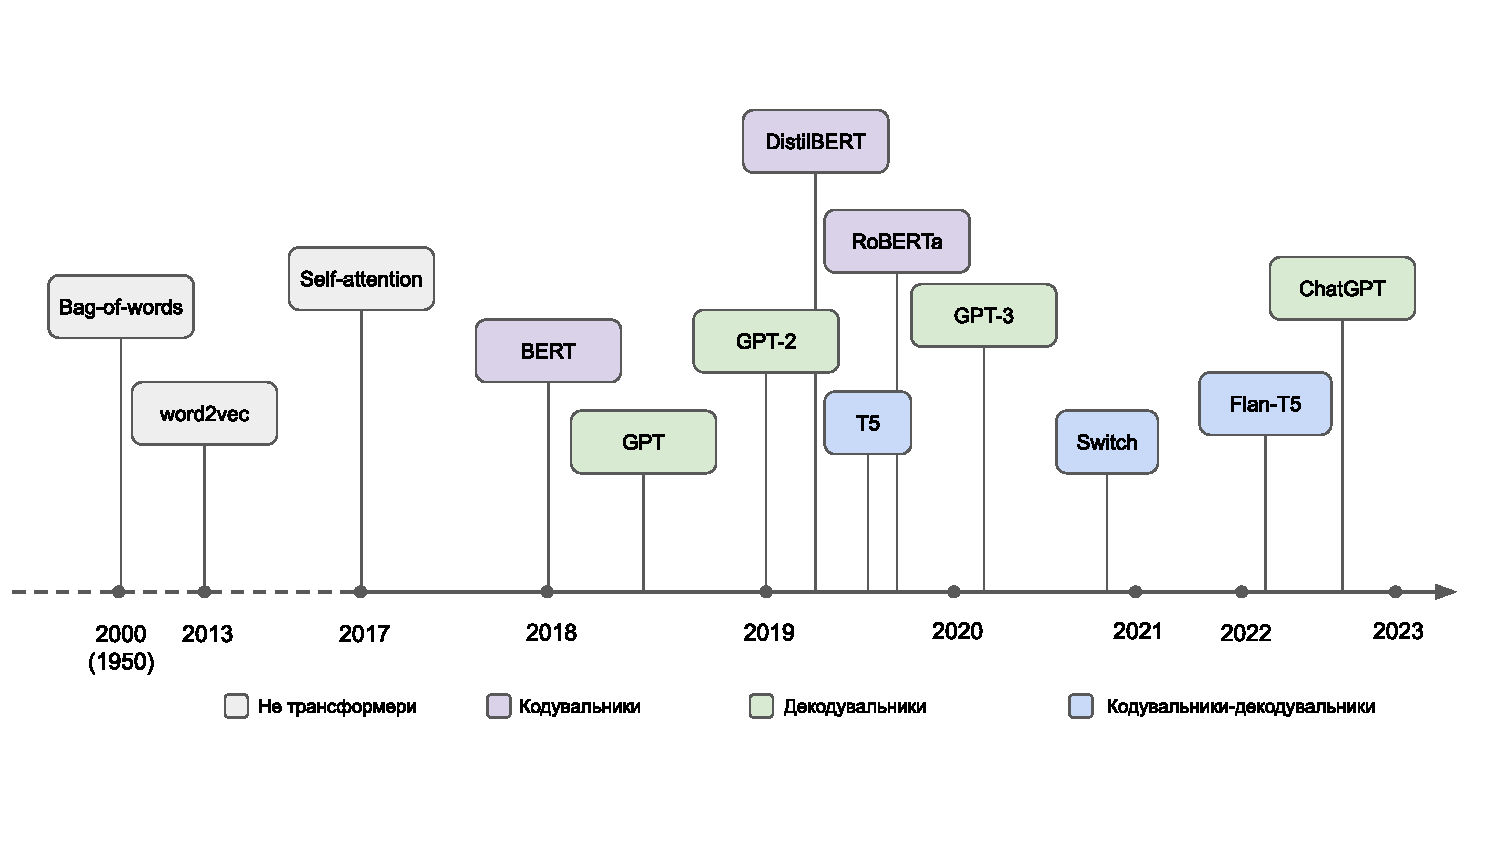
\includegraphics[width=1.0\textwidth]{lang_ai_history.pdf}
    \caption{Історія розвитку методів обробки природної мови за останні 25 років.}
    \label{fig:peek_language_ai}
\end{figure}

Еволюція методів обробки природної мови обумовлена низкою концептуальних і технологічних результатів, спрямованих на розробку систем представлення та генерації природної мови. На рис.~\ref{fig:peek_language_ai} можна бачити історію розвитку NLP у останні 25 років, ілюструючи основні моменти, які поєднують перші спрощені методи з сучасними трансформерними моделями.

Як показано на \ref{fig:lang-ai-tasks}, сучасні технології мовного ШІ застосовуються у широкому діапазоні завдань – від обробки текстового вводу для перекладу до генерації зв’язного тексту в діалогових системах. Оскільки звичайне текстове подання (послідовність чисел) є неструктурованим і втрачає свою смислову інформацію, науковці зосереджують увагу на розробці методів перетворення текстових даних у структуровані числові представлення, що забезпечують ефективну комп'ютерну обробку.

\begin{figure}[!h]
    \centering
    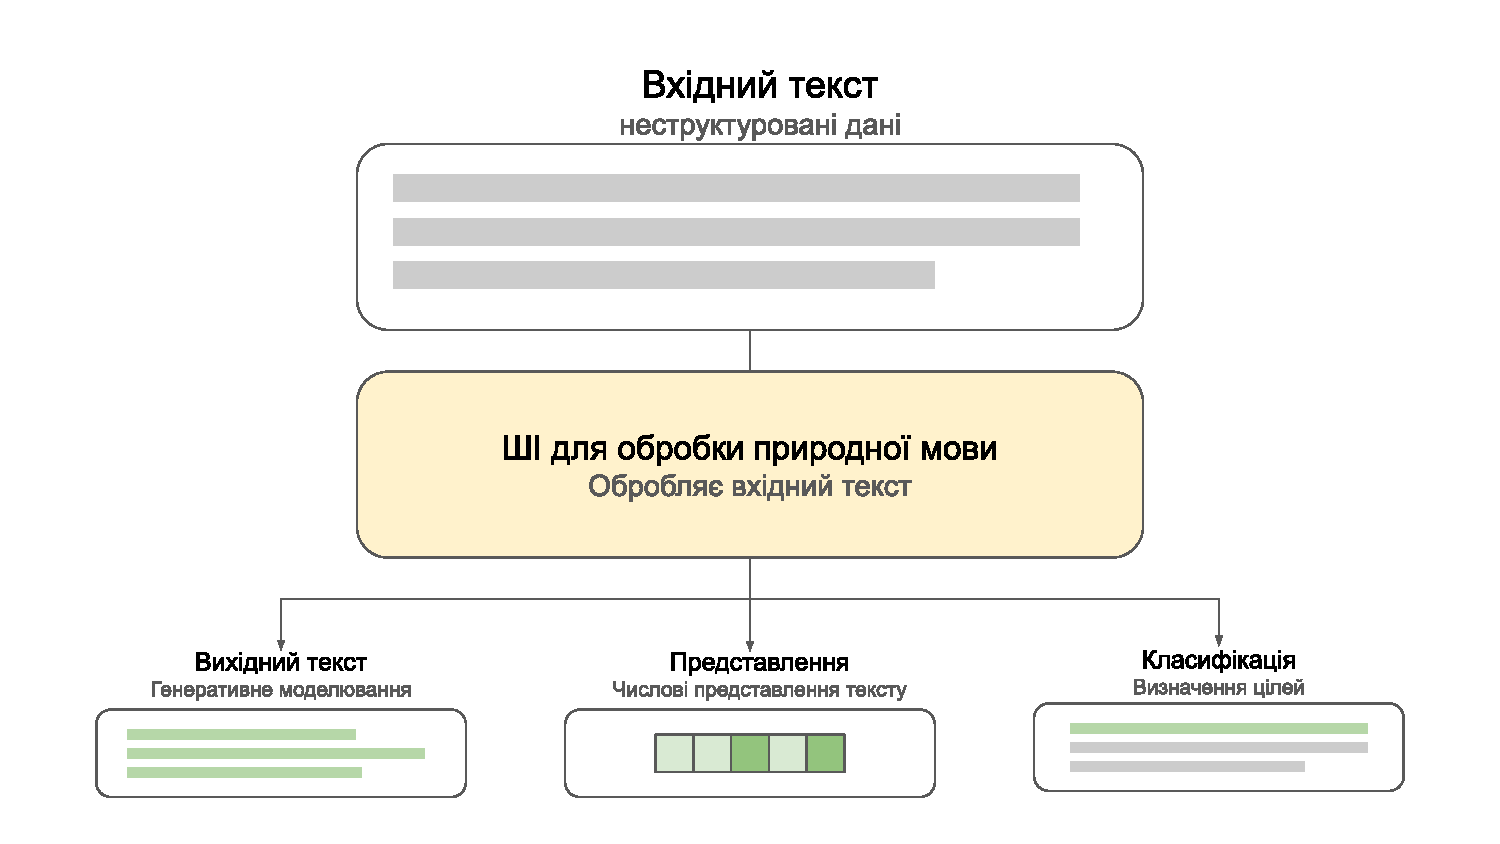
\includegraphics[width=0.8\textwidth]{lang_ai_tasks.pdf}
    \caption{Деякі завдання методів обробки природної мови.}
    \label{fig:lang-ai-tasks}
\end{figure}

\paragraph{Метод мішка слів.}

Перші дослідження в області методів обробки природної мови спиралися на методах представлення тексту без врахування його синтаксичної та семантичної структури або звичайне кодування слів. Метод ``мішка слів'' (bag-of-words), який уперше згадувався ще у 1950-х роках і набув популярності з 2000-х, полягає у перетворенні тексту у вигляді вектору, який утворюється шляхом підрахунку кількості появ кожного унікального слова.

\begin{figure}[!h]
    \centering
    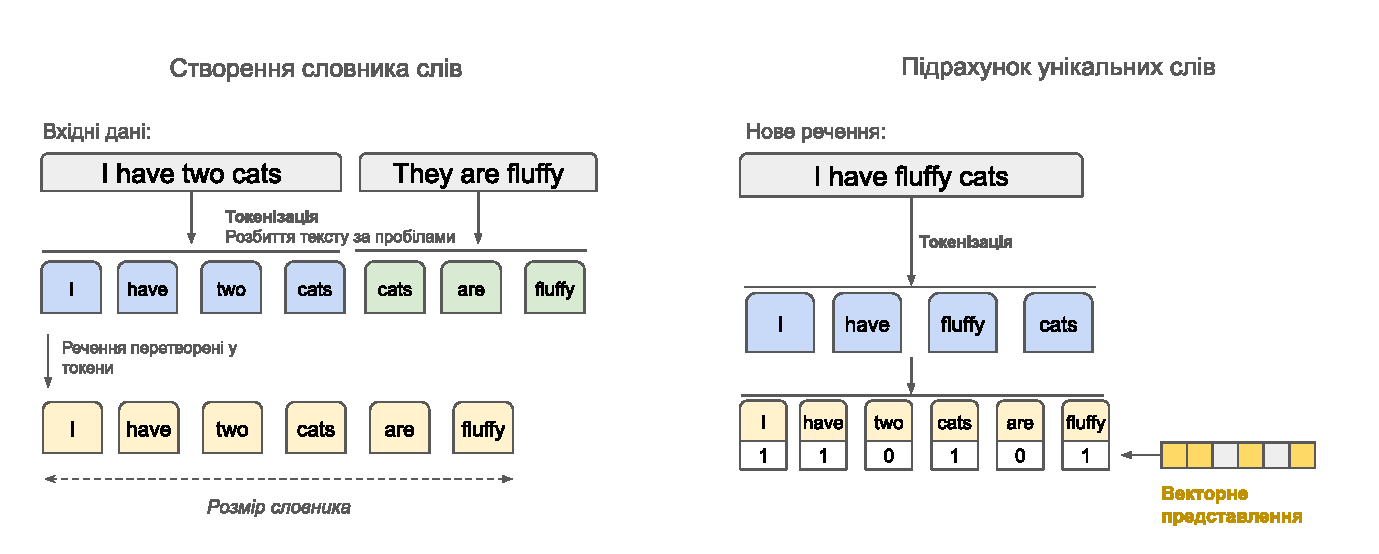
\includegraphics[width=1.0\textwidth]{bow.pdf}
    \caption{Метод ``мішок слів'': токенізація тексту шляхом розбиття за пробілами, формування словника слів та представлення нового вхідного речення у векторному вигляді.}
    \label{fig:bow}
\end{figure}

На рис.~\ref{fig:bow} можна бачити візуалізацію метода ``мішка слів''. На першому кроці відбувається етап токенізації, на якому формується словник з усіх унікальних слів зі вхідних даних. Після цього, коли на вхід отримується нове речення, підрахунок появи кожного слова дозволяє створити векторне представлення тексту за допомогою словника. Попри те, що даний підхід є спрощеним і не відображає семантичну особливості тексту, він заклав основу для подальшого розвитку методів представлення мови.

\paragraph{Векторні представлення слів}
З розвитком методів NLP, почали враховуватися більш динамічні властивості мови, такі як \emph{семантичні (semantic)} та \emph{контекстні (contextual)} особливості слів. Семантика визначає значення слів, фраз і речень незалежно від їхнього текстового оточення, фокусуючись на лексичних та синтаксичних правилах мови. Натомість контекст охоплює мовні та позамовні фактори, що впливають на інтерпретацію значення, зокрема попередні речення, дискурс або інші особливості вживання. Таким чином, семантика забезпечує базове розуміння змісту, тоді як контекст дозволяє враховувати нюанси використання слів та їхнього визначення.

Відповідно наступним кроком у розвитку обробки мовних даних стало використання векторного представлення слів -- \emph{ембединги (word embeggings)}. Метод word2vec, запропонований у 2013 році, полягає в присвоєнні кожному слову фіксованого за розміром вектору, який кодує його семантичні властивості. Це дозволяє за допомогою вимірювання відстаней у векторному просторі оцінювати семантичну подібність між словами.

Процес навчання векторних представлень слів відбувався за допомогою нейронних мереж, які представляють набір шарів та відповідних зв'язків між ними. На кожній ітерації тренування мережа отримує пару слів із текстового корпусу і намагається передбачити, чи є ці слова сусідніми у реченні. В процесі навчання відбувається оптимізація параметрів нейронної мережі (ваги зв'язків), завдяки чому слова з подібними семантичними значеннями отримують близькі ембединги як у прикладі на рис.~\ref{fig:nn_predictions}.

\begin{figure}[!h]
    \centering
    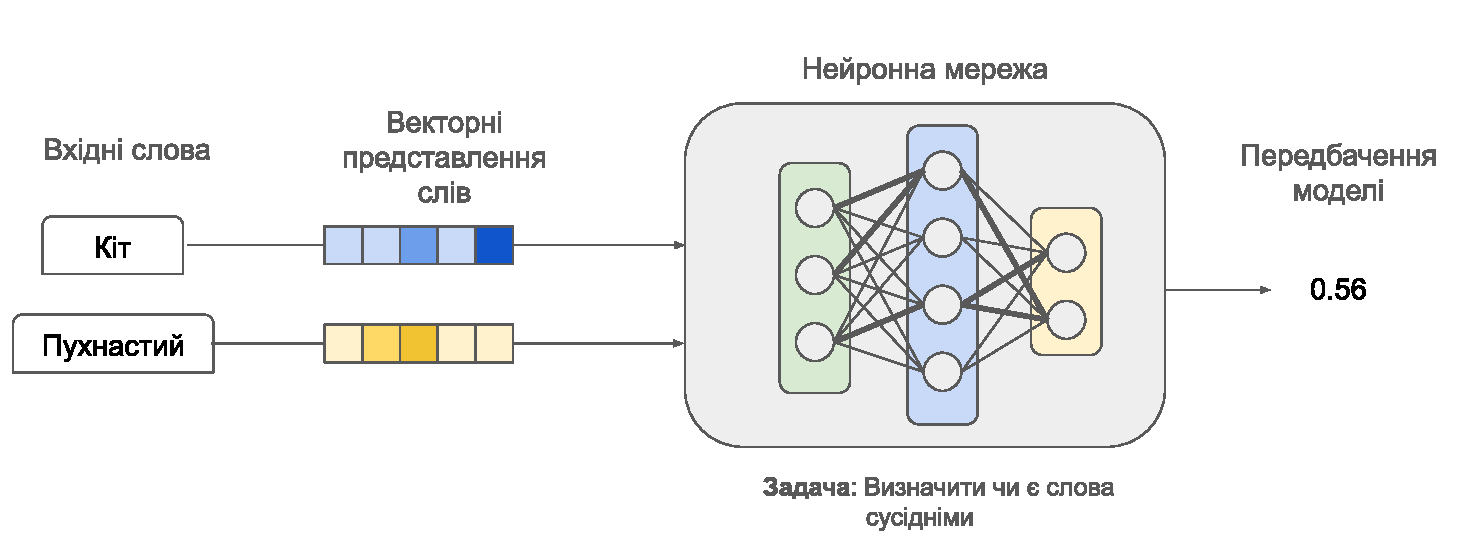
\includegraphics[width=1.0\textwidth]{nn_predictions.pdf}
    \caption{Навчання нейронної мережі шляхом передбачення сусідства слів.}
    \label{fig:nn_predictions}
\end{figure}

Отримані ембединги слів дозволяють описати семантичні властивості слів: наприклад, слово ``кіт'' може набувати високих значень за характеристиками ``тварина'' та ``пухнастість'', тоді як ``гвинтокрил'' матиме низькі значення за цими показниками. Як представлено на рис.~\ref{fig:embeddings} за рахунок векторного представлення відповідні слова можна візуалізувати слів у просторі з метою визначення семантичної близькості між словами.

\begin{figure}[!h]
    \centering
    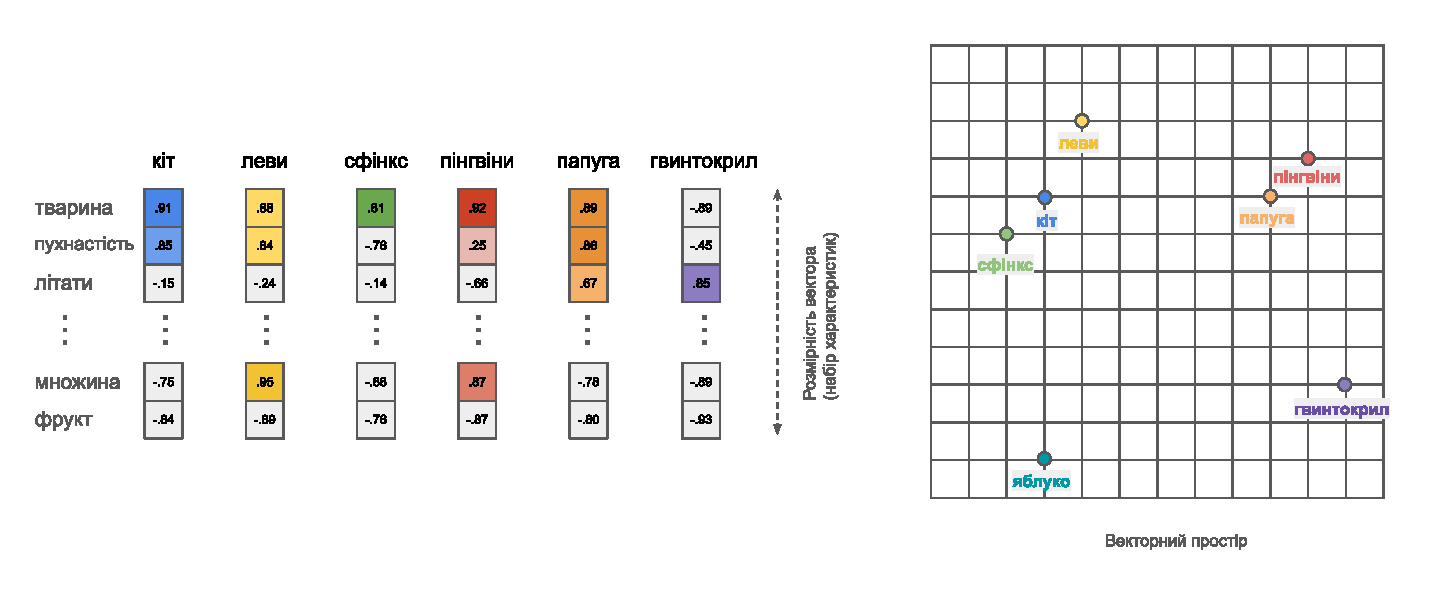
\includegraphics[width=1.0\textwidth]{embeddings.pdf}
    \caption{Ембединги слів, що задають властивості слів та їхня візуалізація у двовимірному просторі. Слова, що мають більше спільних характеристик, знаходяться ближче у просторі.}
    \label{fig:embeddings}
\end{figure}

Слід також зазначити, що існують різні типи векторних представлень даних, що відображають різноманітні рівні абстракції тексту -- від представлення окремих слів до представлення цілих речень або документів.

\paragraph{Кодування та декодування семантики тексту з використанням рекурентних нейронних мереж.}

Перші методи, такі як word2vec, створювали статичні представлення слів, де кожне слово має однаковий вектор значень незалежно від їхньої контекстної інформації (значення слів в залежності від вживання у відповідному реченні). Проте такий підхід не є оптимальним, адже багато слів можуть мати кілька семантичних значень. Наприклад, слово ``замок'' може означати як пристрій для обмеження доступу, так і укріплена будівля

Для врахування семантики слів спочатку застосовувалися рекурентні нейронні мережі (Recurrent Neural Network, RNN). За допомогою RNNs відбувався послідовний процес кодування та декодування заданого тексту. На рис.~\ref{fig:autoregressive_rnn} ілюструється процес генерації перекладу вихідного речення англійською мовою: ``I have two cats'' -- у перекладі українською: ``У мене є два кота''. Даний процес є авторегресійним (autoregressive), тобто кожен попередньо згенерований токен передається на вхід для генерації решти тексту.

\begin{figure}[!h]
    \centering
    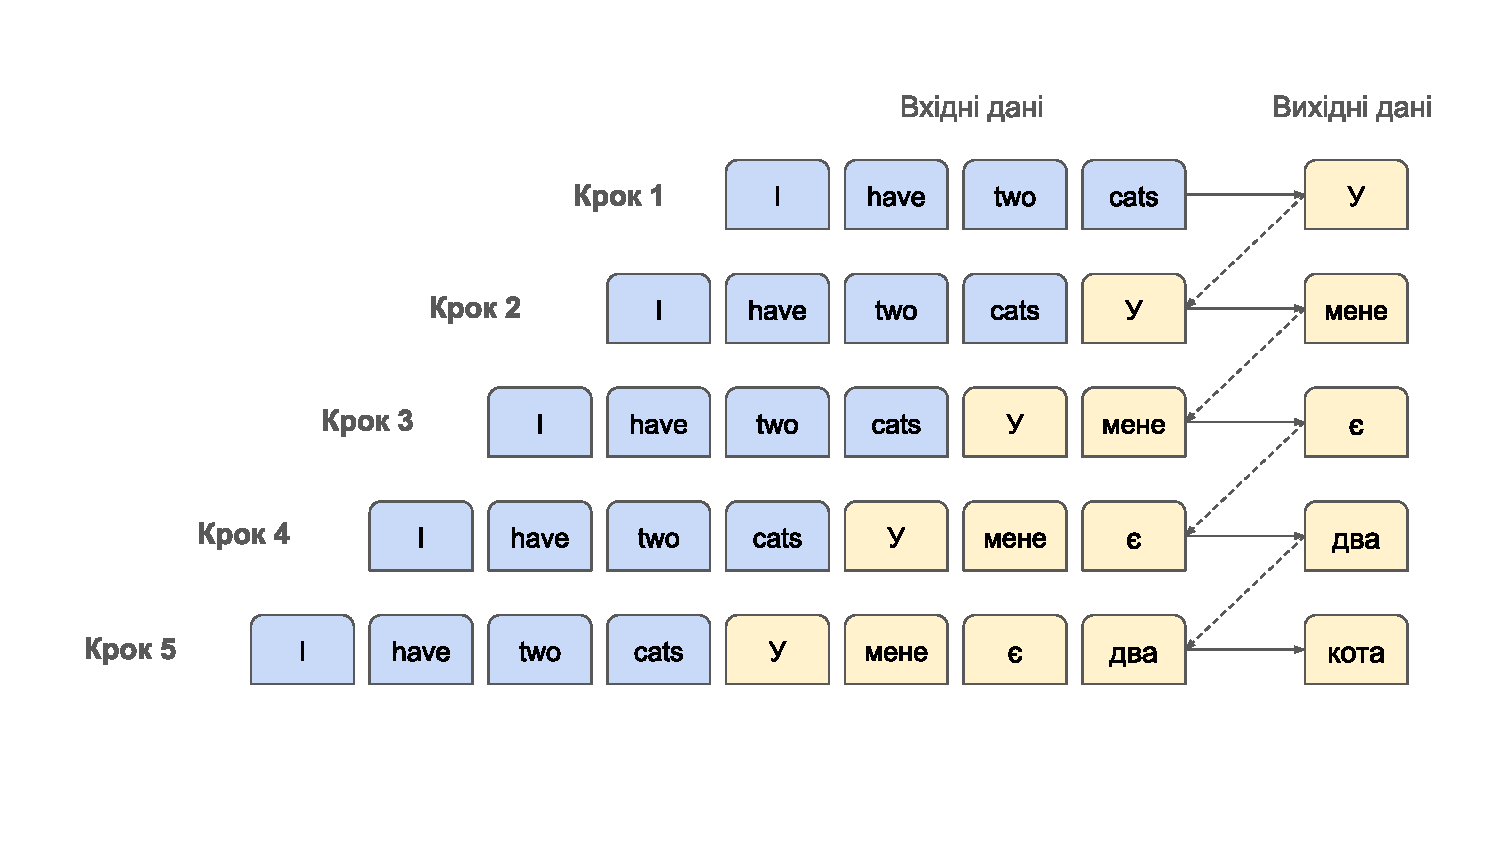
\includegraphics[width=0.9\textwidth]{autoregressive_rnn.pdf}
    \caption{Авторегресійний підхід під час генерації з використанням RNN: Кожен щойно згенерований токен використовується для генерації наступних токенів.}
    \label{fig:autoregressive_rnn}
\end{figure}

У даному методі з метою створення векторного представлення повного речення, на початому етапі були використані ембединги слів методом word2vec, приклад відповідної архітектури та процес обробки вхідного речення можна бачити на рис.~\ref{fig:context_embedding_word2vec}).

\begin{figure}[h]
    \centering
    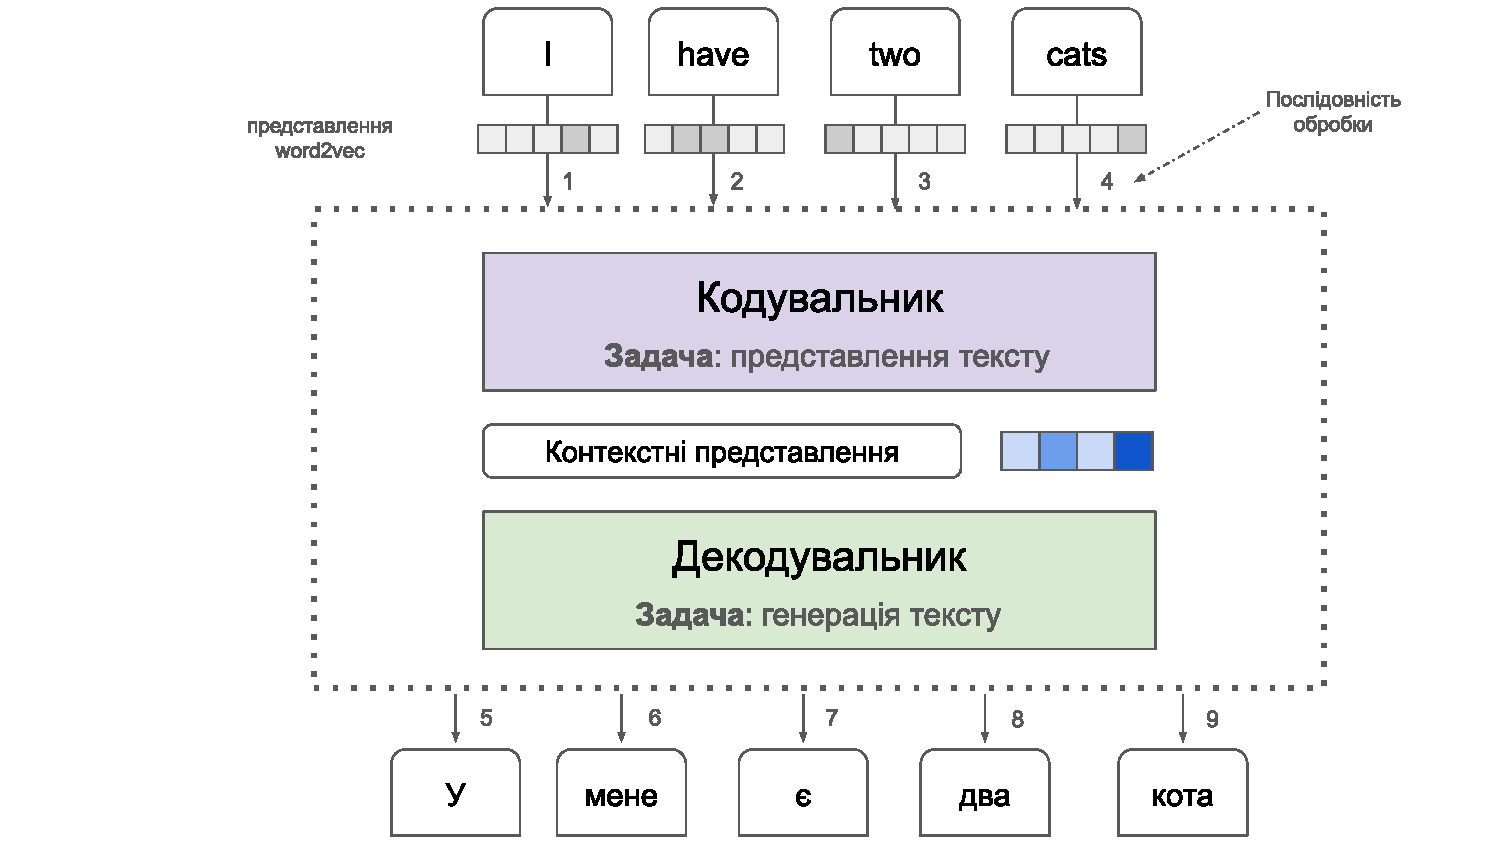
\includegraphics[width=0.9\textwidth]{context_embedding_word2vec.pdf}
    \caption{Формування загального представлення речення на основі векторних представлень слів методом word2vec.}
    \label{fig:context_embedding_word2vec}
\end{figure}

\paragraph{Механізм уваги}
Загальне представлення слів word2vec, як зображено на рис.~\ref{fig:context_embedding_word2vec}, ускладнює обробку речень. Дані ембединги не є чутливими до різноманітного вживання слів при побудові речень, тому відповідно не передають тонкощів задля розуміння текстів. У 2014 році було запропоновано рішення, яке називається \emph{механізм уваги (attention)}, що значно покращило якість векторного представлення текстів. Механізм уваги дозволив моделям зосередитись на частинах речення, які є релевантними до відповідних слів під час побудови перекладу, як зображено на рис.~\ref{fig:attention}. Механізм уваги вибірково визначає, які залежності між словами вхідного та вихідного речення є найбільш суттєвими. Наприклад, вихідне слово ``two'' українською значить ``два'', саме тому ступінь уваги між цими словами є високою. Аналогічно, наприклад, слова ``cats'' та ``мене'' мають нижчий рівень залежності, оскільки вони є менш пов’язаними між собою.

\begin{figure}[h]
    \centering
    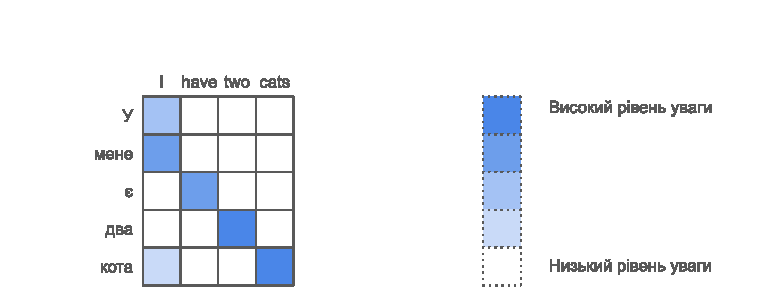
\includegraphics[width=0.9\textwidth]{attention.pdf}
    \caption{Механізм уваги: обчислення взаємозв’язків між токенами для врахування семантичних особливостей слів при побудові векторного представлення.}
    \label{fig:attention}
\end{figure}

Подальше використання механізму уваги у фазі декодування дозволило замість використання єдиного контекстного векторного представлення передавати приховані стани всіх токенів, що значно підвищує якість генерації вихідного тексту.

%%%%%%%%%%%%%%%%%%%%%%%%%%%%%%%%%%%%%%%%%%%%%%%%%%%%%%%%%%%%%%%%%%%%%%%%%%%%%%
\subsection{Модель трансформер}
У роботі "Attention is All You Need" \cite{vaswani2023attentionneed} авторами було представлено модель \emph{трансформер (transformer)}, яка побудована виключно на механізмі уваги і не використовує рекурентні нейронні мережі для обробки тексту. Загальна схема архітектури трансформер складається із набору блоків кодувальників та декодувальників, причому кожен вихідний токен генерується на основі всіх попередніх. Завдяки паралельній обробці токенів цей підхід дозволяє значно скоротити час попереднього тренування моделей та забезпечити отримання більш якісного контекстного значення слів.

Як зображено на рис.~\ref{fig:encoder_block}, кожен кодувальник складається із шару з \emph{механізмом само-уваги (self-attention)}, за яким слідує шар FNN.

\begin{figure}[h]
    \centering
    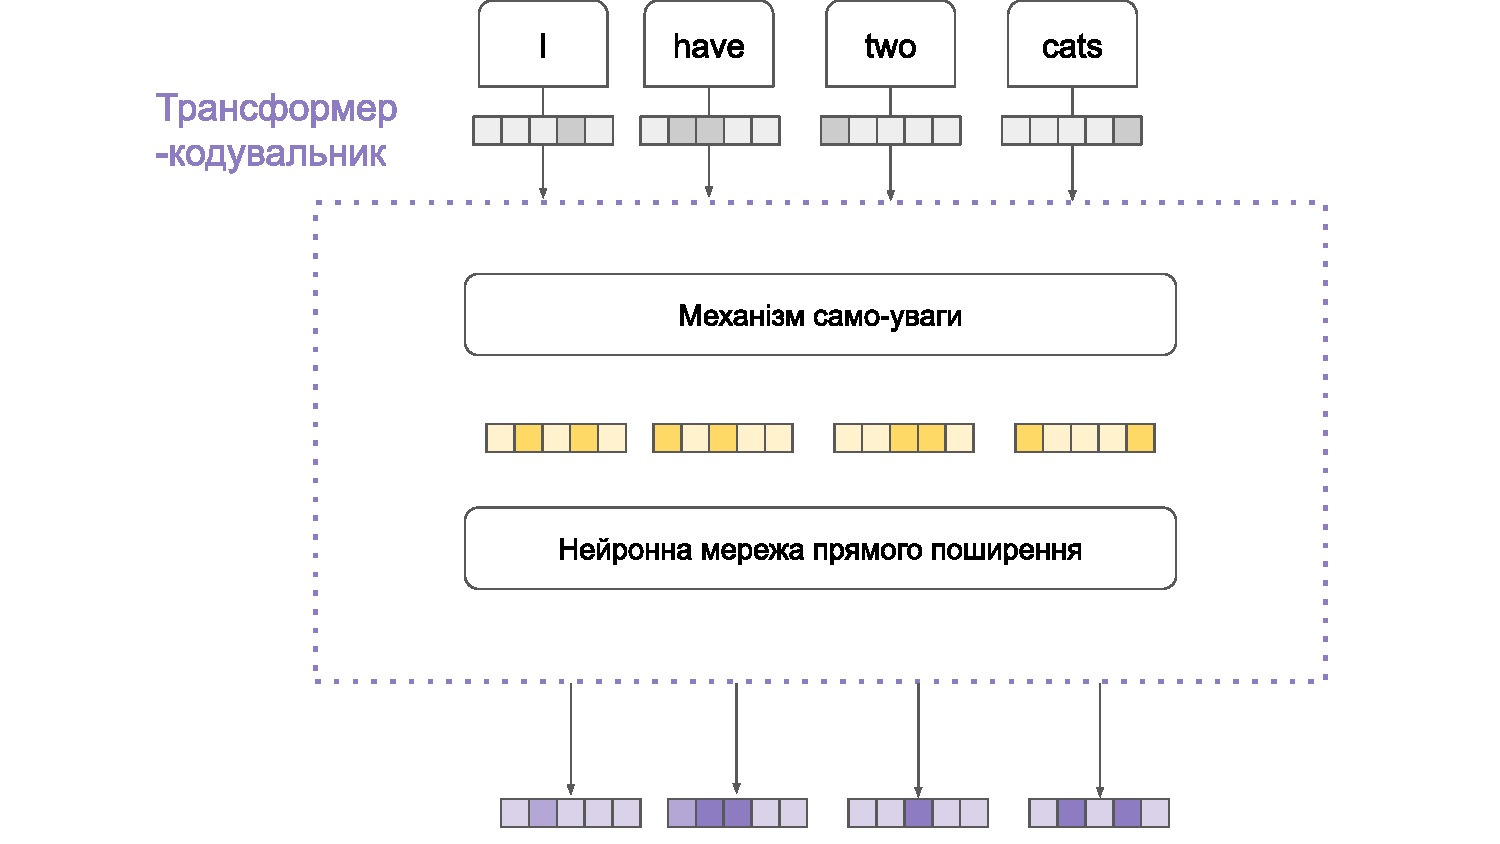
\includegraphics[width=0.9\textwidth]{encoder_block.pdf}
    \caption{Кодувальник моделі трансформер: механізм само-уваги + нейронна мережа прямого поширення.}
    \label{fig:encoder_block}
\end{figure}

Механізм само-уваги дозволяє моделі одночасно аналізувати всі позиції у вхідній послідовності за допомогою декодувальника, який має додатковий рівень уваги, що звертається до вихідних даних кодувальника.

Важливо, що у декодувальнику механізм само-уваги супроводжується маскуванням, щоб запобігати ``зазиранню у майбутнє''.

Наприклад, розглянемо наступне речення:
\begin{lstlisting}[language=json, breaklines=true]
I have two cats, they are fluffy.
\end{lstlisting}

У цьому випадку займенник ``they'' має відношення до слів ``cats'' та ``fluffy''. За допомогою механізму само-уваги модель обчислює вагові коефіцієнти між ``they'' та всіма іншими словами, визначаючи, що саме визначені слова мають найбільше відношення до виділеного слова. На рис.~\ref{fig:self_attention_visualisation} можна бачити взаємозв’язок між токеном ``they'' та рештою токенів у заданому реченні.

% https://colab.research.google.com/drive/1773-ssYunT6oi7vy6hhwwWzj3ibV_Ia5?authuser=1#scrollTo=twSVFOM9SopW
\begin{figure}[h]
    \centering
    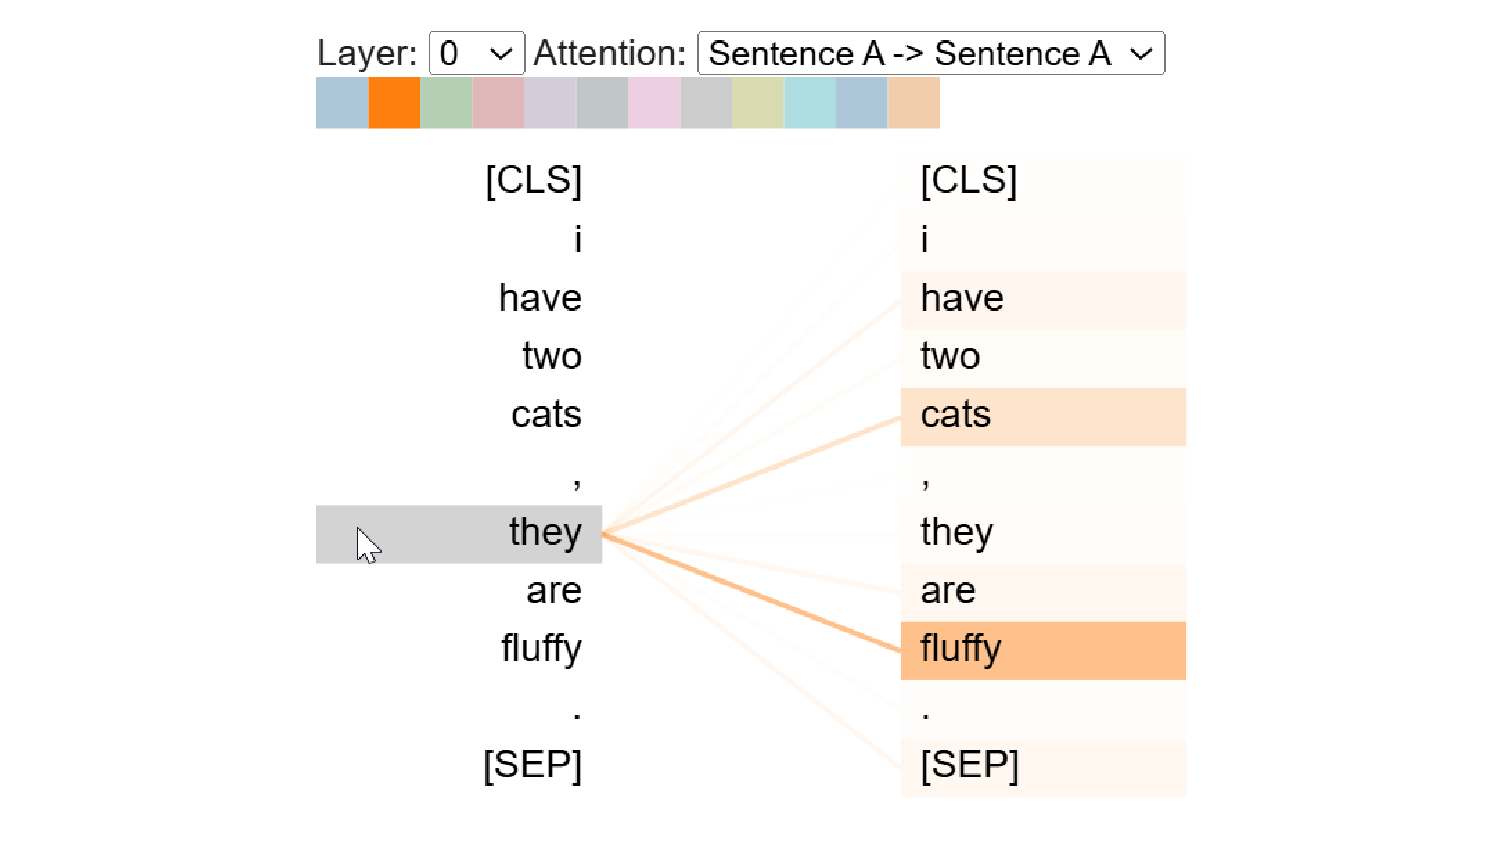
\includegraphics[width=0.6\textwidth]{self_attention_visualisation.pdf}
    \caption{Приклад зв'язків у реченні між токенами за допомогою механізму само-уваги.}
    \label{fig:self_attention_visualisation}
\end{figure}

Слід звернути увагу, що вхід містить додаткові спеціальні токени \texttt{[CLS]} (класифікаційний токен на початку тексту) та \texttt{[SEP]} (токен для ідентифікації кінця речення), які допомагають моделі ефективно обробляти вхідні речення та створювати відповідні представлення. Дані токени також зазвичай використовуються під час тонкого налаштування моделей на конкретних завданнях, таких як класифікація, аналіз тексту та семантичний пошук.

Архітектури, що базуються на моделі трансформер, утворюють основу двох фундаментальних категорій мовних моделей.

\paragraph{Моделі представлення}
Однією з моделей представлення (encoder-only models) є Pre-training of Deep Bidirectional Transformer (BERT) \cite{devlin2019bertpretrainingdeepbidirectional}. Ця модель використовує виключно кодувальні блоки, що складаються з механізму самоуваги та згорткових нейронних мереж, для формування семантичних представлень тексту. Приклад обробки речення за допомогою моделі BERT представлено на рис.~\ref{fig:bert_architecture}.

Додатково для проведення попереднього навчання, використовується крок -- \emph{масковане мовне моделювання (masked language modeling)}, який дозволяє моделі формувати двосторонні представлення, які потім адаптуються для конкретних завдань.

\begin{figure}[h]
    \centering
    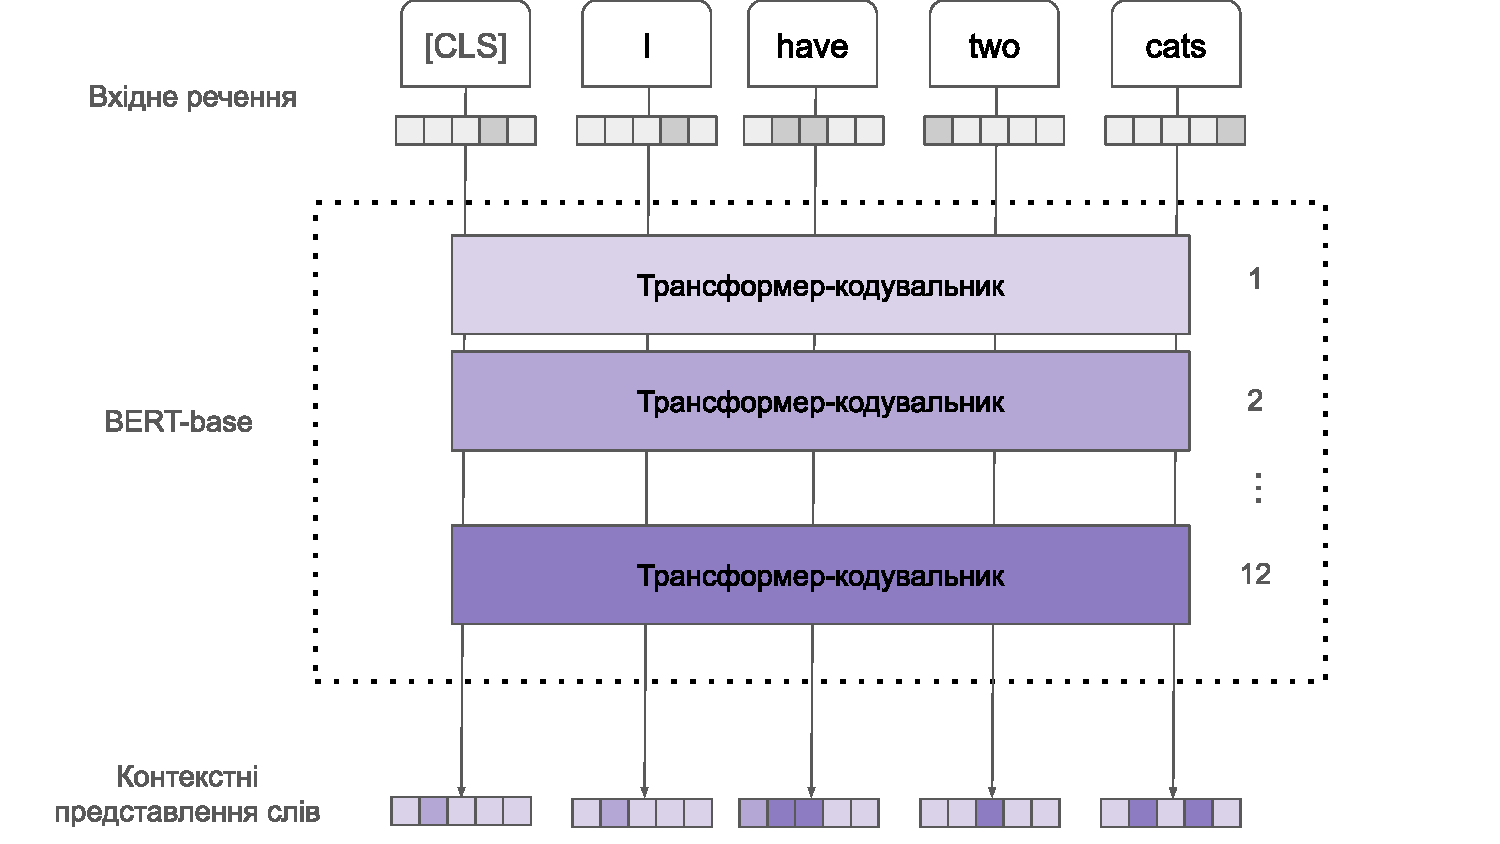
\includegraphics[width=0.9\textwidth]{bert_architecture.pdf}
    \caption{Архітектура базової моделі BERT: 12 кодувальних блоків для генерації представлень.}
    \label{fig:bert_architecture}
\end{figure}

\paragraph{Генеративні моделі.}

Генеративні моделі (decoder-only models), однією з яких є модель генеративного попередньо навченого трансформера (Generative Pretrained Transformer, GPT) \cite{yenduri2023generativepretrainedtransformercomprehensive}. Дана модель оперує виключно за допомогою декодувальних блоків. Завдяки авторегресивному підходу, кожен наступний токен генерується на основі попередніх вхідних даних. Дані системи демонструють високу ефективність у задачах генерації тексту таких як наприклад, написати підсумок тексту, завершити речення, згенерувати відповідь на запитання і тд. Загальний приклад архітектури зображено на рис.~\ref{fig:gpt_architecture}.

\begin{figure}[h]
    \centering
    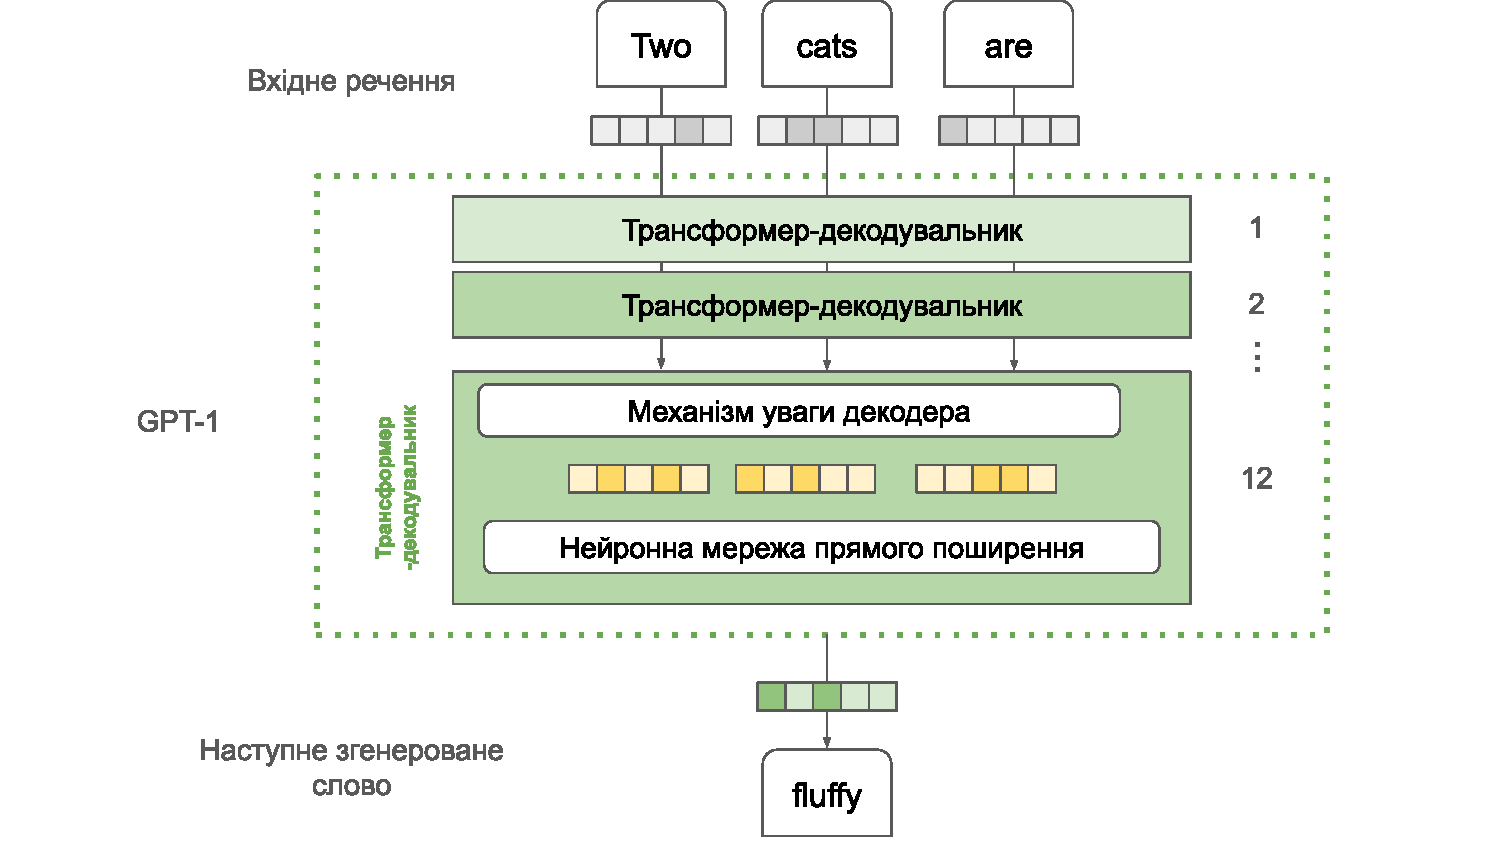
\includegraphics[width=0.9\textwidth]{gpt_architecture.pdf}
    \caption{Архітектура GPT-1: генеративна модель, що використовує лише декодувальник.}
    \label{fig:gpt_architecture}
\end{figure}

На практиці обидва типи моделей (генеративні моделі та моделі представлення) належать до категорії \emph{великих мовних моделей (large language models)}.

Важливою частиною цих моделей завершення є довжина контексту або \emph{контекстне вікно (context window)}. Довжина контексту представляє максимальну кількість токенів, яку модель може обробити, як показано на  рис.~\ref{fig:context_length}. Велике контекстне вікно дозволяє передавати до ВММ на вхід великі об'єми текстових даних. За рахунок авторегресивного підходу роботи цих моделей, поточна довжина контексту під час генерації нових токенів буде збільшуватися. У великих мовних моделях максимальна кількість контекстного вікна обмежується певною кількість токенів, які зазначаються у описі відповідних моделей.

\begin{figure}[h]
    \centering
    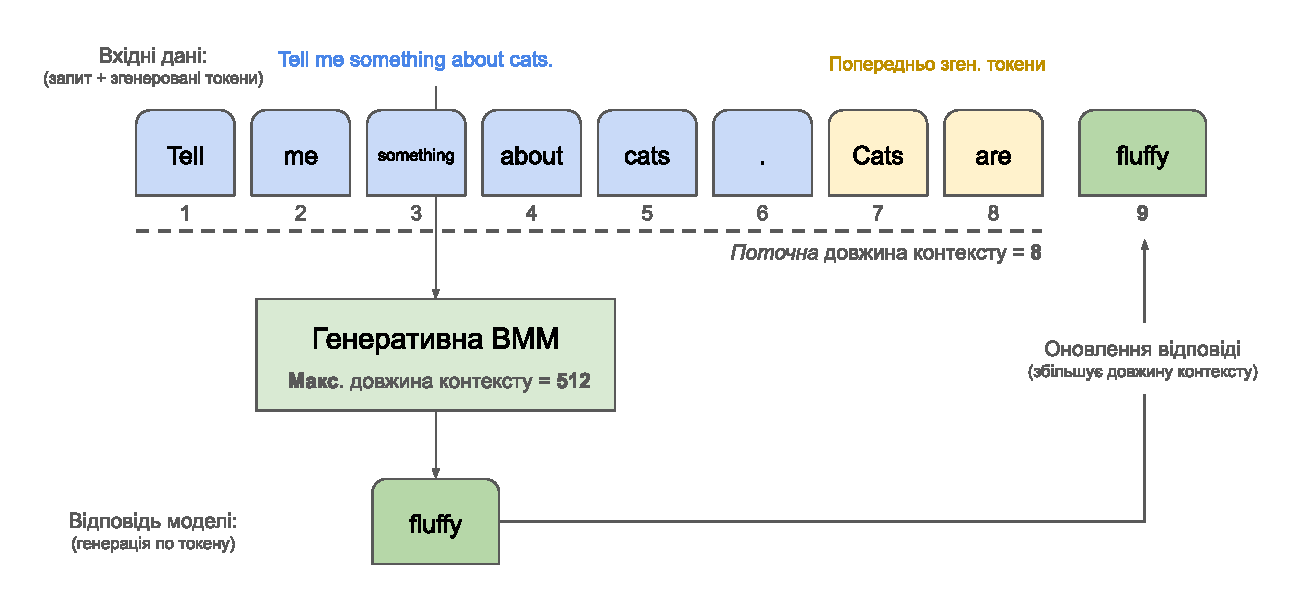
\includegraphics[width=0.9\textwidth]{context_length.pdf}
    \caption{Довжина контекстного вікна -- це максимальна довжина вхідних даних (у токенах), яка може бути оброблена моделлю.}
    \label{fig:context_length}
\end{figure}

%%%%%%%%%%%%%%%%%%%%%%%%%%%%%%%%%%%%%%%%%%%%%%%%%%%%%%%%%%%%%%%%%%%%%%%%%%%%%%
\subsection{Великі мовні моделі}

\paragraph{Парадигма тренування великих мовних моделей}

\begin{figure}[h]
    \centering
    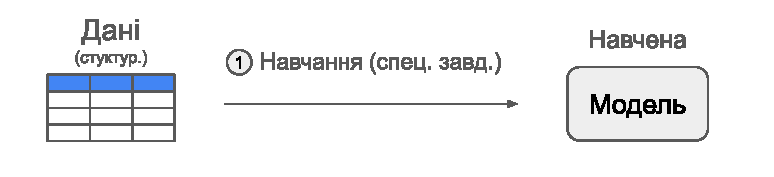
\includegraphics[width=0.6\textwidth]{ml.pdf}
    \caption{Традиційне машинне навчання включає один крок: навчання моделі для конкретного цільового завдання, наприклад, класифікації чи регресії.}
    \label{fig:ml}
\end{figure}

На відміну від традиційних методів машинного навчання, що базуються на навчанні моделей для виконання певного завдання -- рис.~\ref{fig:ml}, розробка ВММ передбачає багатоступеневий підхід. 
\begin{figure}[h]
    \centering
    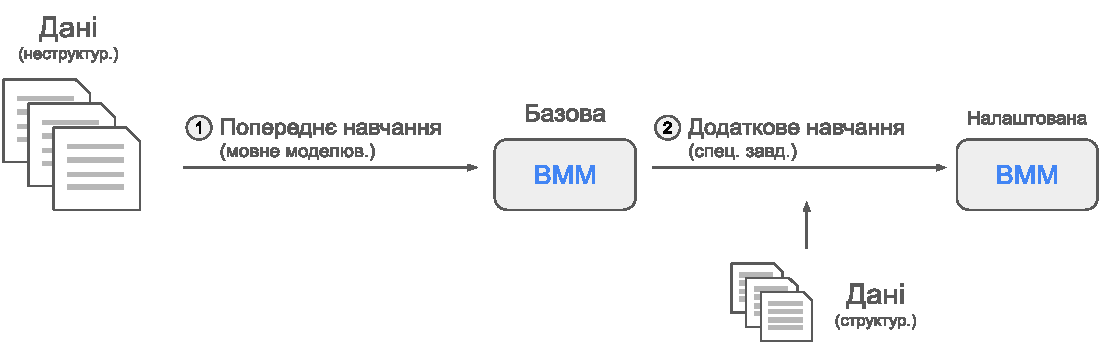
\includegraphics[width=0.9\textwidth]{llm_training.pdf}
    \caption{Багатокроковий процес навчання ВММ: попереднього тренування та тонкого налаштування.}
    \label{fig:llm_training}
\end{figure}

Як можна бачити з рис.~\ref{fig:llm_training}, типовий процес навчання сучасних трансформерних ВММ \cite{ouyang2022traininglanguagemodelsfollow} складається з трьох основних етапів:

\begin{enumerate}

    \item {Попереднє тренування (Pre-training)}
    На цьому етапі ВММ тренуються на великих корпусах текстів, щоб засвоїти загальні закономірності мови, граматику, семантичні зв’язки між елементами тексту з урахуванням особливостей відповідного завдання. Отримана ``базова'' модель є вихідною точкою для подальшої адаптації та удосконалення моделі на відповідних задачах. За рахунок попереднього тренування моделі вчаться прогнозувати наступний токен по заданому вхідному тексті. На рис.~\ref{fig:pretraining} зображено процес попереднього тренування моделі на корпусі даних Common Crawl.
    
    \item {Тонке налаштування (Fine-tuning)}
    На цьому етапі базову модель далі адаптують для виконання вузько-направлених завдань (класифікація, інформаційний пошук, генерація діалогів тощо), що дозволяє значно знизити обчислювальну вартість. Цей підхід, представлений на \ref{fig:llm_training}, є стандартним у сучасних методах розробки ВММ. Одним з різновидів додаткового навчання є кероване навчання (supervised fine-tuning), при якому моделі додатково навчаються на парах інструкція-відповідь, щоб покращити виконання спеціалізованих завдань.
    
    \item {Вирівнювання (Alignment)}: Додатковим етапом сучасних мовних моделей також є етап вирівнювання, під час якого моделі налаштовуються для більш корисних та безпечних відповідей на основі людського зворотного зв'язку. Задля цього використовуються такі методи як RLHF, про які буде розповідатися детальніше у одному з наступних розділів.
    
\end{enumerate}

% джерело: https://cameronrwolfe.substack.com/p/language-models-gpt-and-gpt-2
\begin{figure}[h]
\centering
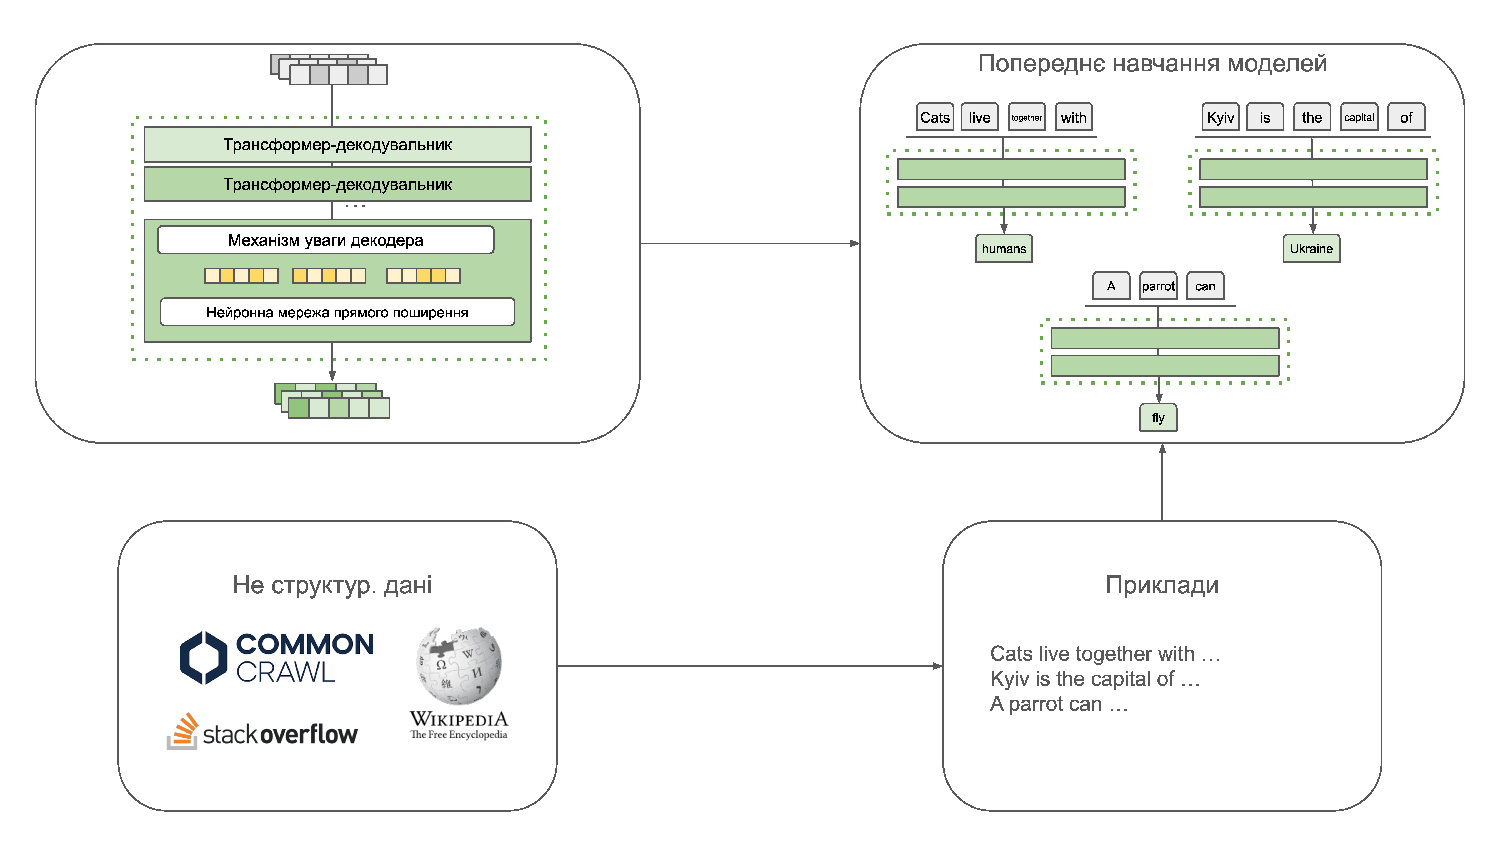
\includegraphics[width=0.9\textwidth]{llm_pretraining_step.pdf}
\caption{Ілюстрація етапу попереднього тренування ВММ.}
\label{fig:pretraining}
\end{figure}

\paragraph{Новітні тенденції та їх вплив на практику}
Останнім часом, особливо в 2022–2023 роках, технології на базі трансформерних моделей отримали значний вплив завдяки появі систем, що кардинально змінюють взаємодію користувачів з інформаційними технологіями. Швидке зростання активних користувачів, широке застосування мовного ШІ у різних галузях (від машинного перекладу до генерації контенту) сприяє подальшим інноваціям у цій сфері, а також вивченню етичних та соціальних наслідків впровадження таких технологій.

\paragraph{Застосування ВММ та соціально-етичні виклики.}

Великі мовні моделі мають застосування в багатьох галузях: від визначення тональності клієнтських відгуків (класифікація) до розробки інтерактивних чат-ботів, що використовують зовнішні інформаційні джерела для підвищення якості відповідей. Сучасні мультимодальні системи, зокрема генерація рецептів за зображенням вмісту холодильника, демонструють високий рівень інноваційності цих технологій.

Однак широке впровадження ВММ супроводжується й низкою соціально-етичних викликів. До них належать питання упередженості даних, проблеми прозорості алгоритмічних та архітектурних рішень, потенційна генерація шкідливого або дезінформаційного контенту, а також питання інтелектуальної власності. Врахування цих аспектів є необхідним для безпечного та відповідального використання технологій мовного ШІ.

ВММ, такі як GPT-4, демонструють значні здібності до розуміння та генерації математичних текстів, що відкриває можливості для їх використання у задачах математичного міркування \cite{openai2024gpt4technicalreport}.

Для подальшого удосконалення роботи ВММ з математичними текстами існує кілька методів, які наведені у наступному підрозділі.

%%%%%%%%%%%%%%%%%%%%%%%%%%%%%%%%%%%%%%%%%%%%%%%%%%%%%%%%%%%%%%%%%%%%%%%%%%%%%%
\section{Сучасні архітектури та методи для підвищення ефективності великих мовних моделей}

% https://huggingface.co/blog/moe
\subsection{Модель зі змішанням експертів}

Вперше ідея моделей зі змішанням експертів (MoE) була запропонована ще у 1991 році у роботі \textit{Adaptive Mixture of Local Experts} \cite{6797059}. Основна концепція MoE полягає в розбитті великої моделі на окремі моделі меншого розміру, яка отримали назву моделей-експертів або просто \emph{експертів (experts)}, кожен з яких спеціалізується на обробці певної підмножини завдань або видів вхідних даних. Вибір конкретного експерта або комбінації експертів здійснюється за допомогою спеціалізованого \emph{маршрутизатора (router)}, що визначає, яких із експертів активувати для обробки відповідного вхідного запиту.

У період між 2010-2015 роками архітектура з використанням MoE охоплювала два основних напрямки досліджень:
\begin{itemize}
    \item {Експерти як компоненти моделі}: Дані методи передбачали використання кількох незалежних моделей нейронних мереж, результати яких агрегувалися для отримання остаточного результату. Автори \cite{eigen2014learningfactoredrepresentationsdeep} пропонують інтеграцію MoE як окремого шару моделі, з використанням експертів, які спеціалізуються на обробці конкретних типів вхідних даних.
    \item {Умовні обчислення}: Традиційні щільні нейронні мережі (Dense Neural Networks) використовують всі параметри всіх шарів для обчислення результатів. Тому як більшу альтернативу \cite{bengio2016conditionalcomputationneuralnetworks} було запропоновано ефективне використання нейронної мережі, що дозволяє активувати лише певну підмножину параметрів залежно від особливостей вхідних даних. Таким чином, модель використовує лише частину параметрів нейронної мережі моделі, але при цьому має не гіршу та не рідко навіть кращу ефективність у порівнянні з моделями подібного розміру.
\end{itemize}

Загальний вигляд архітектури з використанням MoE-шару наведено на рис.~\ref{fig:moe-layer}.

\begin{figure}[!h]
    \centering
    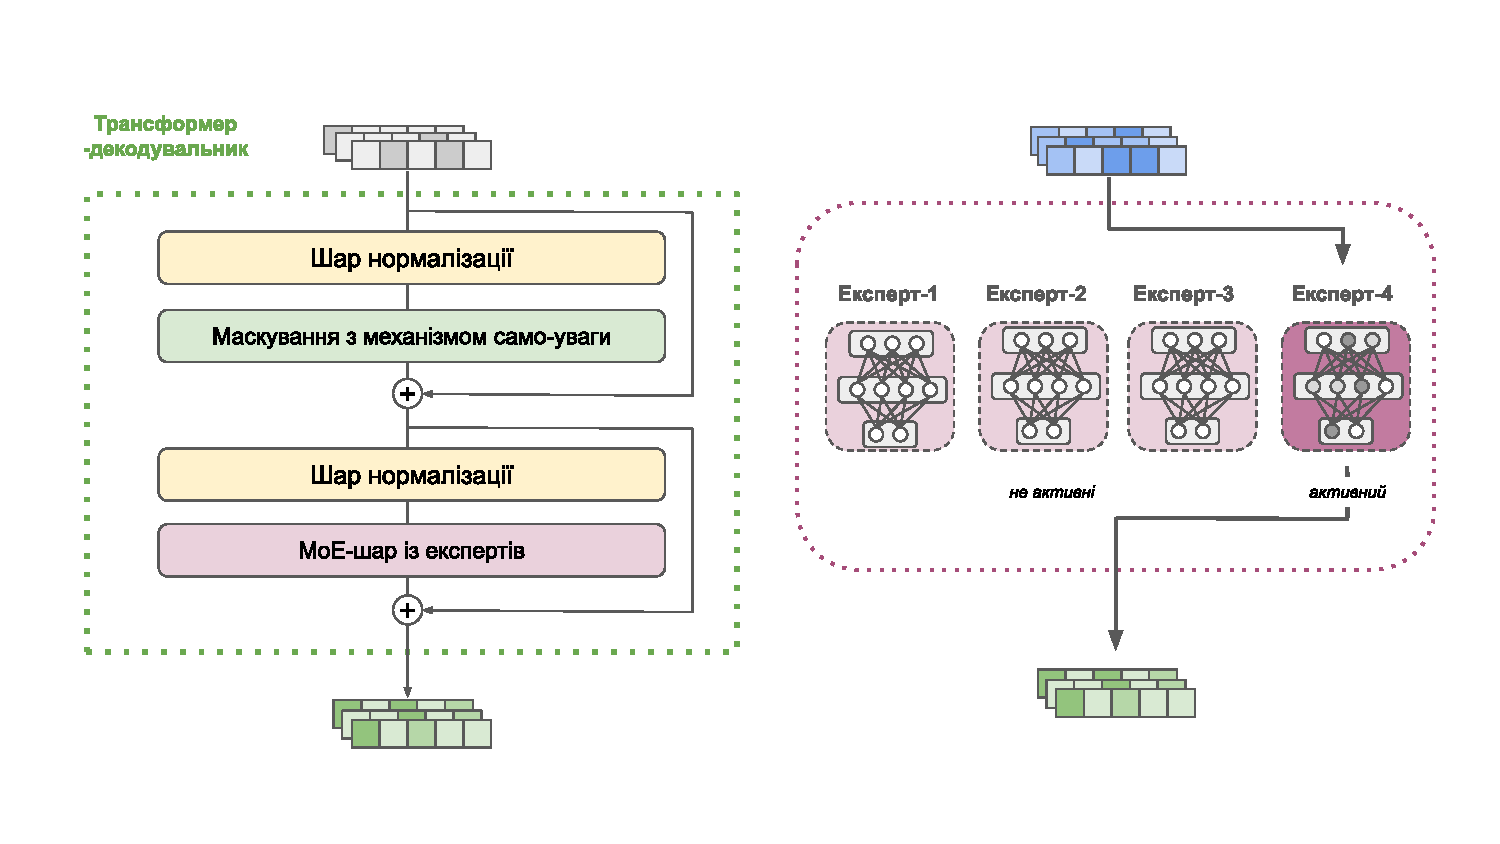
\includegraphics[width=0.9\textwidth]{moe_layer.pdf}
    \caption{MoE-шар моделі.}
    \label{fig:moe-layer}
\end{figure}

Після цього модель почали активно використовувати у задачах з NLP. Але спочатку визначимо поняття розрідженості (sparsity) у моделях.

\paragraph{Розрідженість у MoE}
Розрідженість моделей базується на ідеї використання умовних обчислень, при яких лише частина мережі активна в залежності від вхідних даних, що дозволяє збільшувати розмір моделі без збільшення обчислень, що дозволяє використовувати велику кількість експертів у кожному окремому шарі MoE.

Однак, ця конфігурацію створює певні виклики. Наприклад, якщо пакетний вхід складається з 10 токенів, п'ять токенів можуть потрапити до одного експерта, а інші п'ять -- до п'яти різних експертів, що призводить до нерівних розмірів розподілу вхідних даних.

Для вирішення цієї проблеми використовується навчена мережа маршрутизатор ($G$), яка вирішує, до яких експертів ($E$) відправити вхідний запит:

\begin{equation}
    y = \sum_{i=1}^{n} G(x)_i E_i(x)
\end{equation}

У даній конфігурації всі експерти запускаються для всіх входів. Якщо для деякого з експертів значення $G_i=0$, обчислення відповідного експерта не використовуються, і таким чином запобігається використання відповідних обчислювальних ресурсів. Зазвичай у якості функції активації мережі маршрутизатора використовується softmax. Мережа навчається визначати, до якого експерта відправити вхід:

\begin{equation}
    G_{\sigma}(x) = \text{Softmax}(x \cdot W_g)
\end{equation}

Інший підхід, який наприклад досліджувався у роботі \cite{shazeer2017outrageouslylargeneuralnetworks} -- Noisy Top-k Gating. Цей підхід вводить регульований шум і зберігає топ-$k$ значень:

Це робиться за рахунок додавання шуму:

\begin{equation}
    H(x)_i = (x \cdot W_g)_i + \text{StandardNormal()} \cdot \text{Softplus}((x \cdot W_{\text{noise}})_i)
\end{equation}

Після чого обираються лише топ-$k$ значення:

\begin{equation}
    \text{KeepTopK}(v, k)_i = \begin{cases}
        v_i, & \text{якщо } v_i \text{ входить до топ } k \text{ елементів } v, \\
        -\infty, & \text{інакше}
    \end{cases}
\end{equation}

І далі використовується softmax від отриманого результату:

\begin{equation}
    G(x) = \text{Softmax}(\text{KeepTopK}(H(x), k))
\end{equation}

Оскільки розрідженість керована параметром $k$, вона має додаткові особливі властивості. Використовуючи досить низьке $k$, можна тренувати та виконувати висновок набагато швидше, ніж при активації багатьох експертів. Маршрутизація до більше ніж одного експерта необхідна для того, щоб маршрутизатор навчився розподіляти вхідний запит між кількома експертами.

Додавання шуму сприяє балансуванню навантаження. Якщо всі токени надсилаються до лише декількох популярних експертів, тренування може призвести до нерівномірного тренування моделей. Це відбувається на етапі попереднього тренування MoE-моделі, коли маршрутизатор обирає схожих експертів за рахунок того, що обрані експерти тренуються швидше і тому вибираються частіше. Щоб уникнути цього, додається допоміжна функція втрат, яка заохочує рівномірний розподіл використання експертів. Ця функція втрат гарантує, що всі експерти отримують приблизно однакову кількість навчальних прикладів.

\paragraph{MoE та моделі трансформери}
У трансформерних моделях MoE застосовуються як шари, що замінюють звичайні шари щільних нейронних мереж прямого поширення. Структура такого шару MoE складається з двох основних компонентів:
\begin{enumerate}
    \item {Шарів експертів}: кожен експерт зазвичай реалізується у вигляді окремого шару FNN, що відповідає за обчислення для певної підмножини вхідних токенів. Структура експертів може відрізнятися, проте існують варіанти, коли експерти реалізуються як більш складні мережі або як набір експертів, що дозволяє моделі комплексно адаптуватися до різних типів даних.
    \item {Маршрутизатор}: цей компонент аналізує вхідний токен (або його представлення) і за допомогою функції softmax розраховує вагові коефіцієнти для кожного експерта. Таким чином, маршрутизатор вибирає топ-$k$ експертів (часто $k=1$ або $2$) для обробки даного токена. Такі підходи, як Noisy Top-$k$ Gating, вводять регульований шум для балансування навантаження між експертами та зниження надмірної спеціалізації окремих модулів.
\end{enumerate}

Завдяки даному підходу при обробці кожного вхідного прикладу активуються лише частина експертів, що дозволяє збільшувати модель до значно більшої кількості параметрів без активації усіх параметрів моделі. У зв'язку з цим такі моделі також називають розрідженими (sparse), адже при роботі моделей використовується лише частина параметрів.

\paragraph{Приклади моделей MoE}
Одним із прикладів застосування MoE у трансформерних моделях є Switch Transformers \cite{fedus2022switchtransformersscalingtrillion}. У цій моделі щільні FNN-шари звичайного трансформера замінюються розрідженими MoE-шарами. Кожен MoE-шар може складатися з декількох експертів, проте для кожного входу активується лише частина експертів, що значно знижує обчислювані навантаження під час генерації вихідних даних. Моделі даного типу дозволили досягнути чотирикратного прискорення попереднього тренування моделі у порівнянні зі щільними архітектурами, але при цьому зберігаючи високу якість результатів.

Іншим прикладом є система GShard \cite{lepikhin2020gshardscalinggiantmodels}, де розріджені MoE-шари інтегровані в трансформерну архітектуру для збільшення моделі до понад 600 мільярдів параметрів. У цій системі шари MoE розподіляються між різними пристроями, що дозволяє ефективно використовувати обчислювальні ресурси при обробці великих обсягів тренувальних даних.

Таким чином, інтеграція MoE в трансформерні архітектури має ряд важливих переваг:
\begin{itemize}
    \item {Ефективне збільшення моделей}: При збереженні однакових обчислювальних затрат розріджена модель MoE містить значно більше параметрів, ніж щільна модель, що дозволяє використовувати набагато більше даних і підвищувати якість попереднього тренування моделей.
    \item {Умовні обчислення}: Завдяки маршрутизатору активуються лише релевантні експерти для кожного вхідного запиту, що дозволяє зменшити обчислювальні витрати.
    \item {Спеціалізація експертів}: Кожен експерт може адаптуватися до обробки певних типів вхідних даних, що сприяє кращому моделюванню складних семантичних залежностей у відповідних даних.
\end{itemize}

Слід зазначити, що згідно із дослідженнями у використанні архітектури MoE у моделях (наприклад, \cite{xue2024openmoeearlyeffortopen}) різні експерти не спеціалізуються на конкретних темах, таких як біологія, математика тощо. Проте працюють з певними наборами токенів, які подаються на вхід моделей. Як результат -- моделі схильні категоризувати роботу з певними природними мовами (наприклад, англійська, українська), адже вони несуть свої особливості у символьному представленні слів. Орієнтованість на вибір відповідних задач можна бачити при перегляді найбільш активно вживаних токенів відповідними експертами, як наведено у таблиці~\ref{tab:top_token_table}.

\begin{figure}[h]
    \centering
    \captionof{table}{Найчастіше вживані токени, що використовуються різними експертами \cite{xue2024openmoeearlyeffortopen}.}
    \label{tab:top_token_table}
    \begin{tabular}{|c|l|}
        \hline
        ID експерта & Найбільш активно вживані токени \\
        \hline
        0 & \hlblue{\textbackslash n}, \hlblue{`}, \hlblue{’}, \hlblue{s}, \hlblue{-}, \hlblue{\$}, \hlblue{y}, \hlblue{\_}, \hlblue{\,}, \hlblue{2} \\
        1 & \hlgreen{\textbackslash n}, \hlgreen{1}, \hlgreen{\,}, \hlgreen{2}, \hlgreen{\textbackslash\textbackslash}, \hlgreen{S}, \hlgreen{.}, \hlgreen{-}, \hlgreen{C}, \hlgreen{\{} \\
        21 & \hlred{,}, \hlred{and}, \hlred{\,}, \hlred{.}, \hlred{\textbackslash n}, \hlred{=}, \hlred{\textbackslash t}, \hlred{the}, \hlred{\,}, \hlred{n} \\
        30 & \hlpurple{\}}, \hlpurple{ed}, \hlpurple{d}, \hlpurple{have}, \hlpurple{ing}, \hlpurple{,}, \hlpurple{has}, \hlpurple{s}, \hlpurple{\"}, \hlpurple{had} \\
        31 & \hlgrey{to}, \hlgrey{can}, \hlgrey{s}, \hlgrey{of}, \hlgrey{ing}, \hlgrey{will}, \hlgrey{not}, \hlgrey{e}, \hlgrey{ed}, \hlgrey{would} \\
        \hline
    \end{tabular}
\end{figure}


Однак, моделі зі змішанням експертів мають свої недоліки, зокрема:
\begin{itemize}
    \item {Балансування навантаження}: Одні експерти можуть активуватися частіше, що призводить до нерівномірного розподілу обчислювальних ресурсів та їхнього потенційного перенавчання (overfitting).
    \item {Супутні обчислювальні та комунікаційні витрати}: Хоча під час висновку активуються лише обрані експерти, всі параметри повинні бути завантажені в оперативну пам’ять, що може створювати додаткові вимоги до апаратного забезпечення.
\end{itemize}

Щоб вирішити ці проблеми, застосовуються такі методи, як додавання надмірного шуму до маршрутизатора та додаткові функції втрат (loss function), які стимулюють рівномірний розподіл навантаження між моделями-експертами. Також застосовуються методи умовної маршрутизації, що дозволяють ефективно задіювати обчислювальний ресурс при навчанні та генерації відповідей.

У підсумку, MoE представляють собою потужний підхід для збільшення параметрів трансформерних архітектур із збереженням обчислювальної ефективності та високої якості моделі. Нижче наведені деякі приклади моделей, які ілюструють практичне застосування цієї ідеї в сучасних системах обробки природної мови та їх порівняння з традиційними моделями, що використовують щільні нейронні мережі.

\paragraph{Приклади моделей з використанням MoE}
Після обґрунтування концепції MoE, розглянемо кілька прикладів даних моделей. Завдяки тому, що великі мовні моделі збільшують ефективність своєї роботи при збільшенні параметрів, MoE були широко впроваджені і досягли успіху у дослідженнях з ВММ.

Одним з прикладім моделей з використанням MoE є Mixtral 8×7B (Mixtral of Experts \cite{jiang2024mixtralexperts}) та є розширенням для відкритої моделі Mistral-7B \cite{jiang2023mistral7b}, яка володіє англійською, французькою, італійською, німецькою та іспанською мовами. Обидві ці моделі мають оприлюднені ваги та інші специфікації задля відкритого користування розробниками та дослідниками.

\begin{figure}[h]
    \centering
    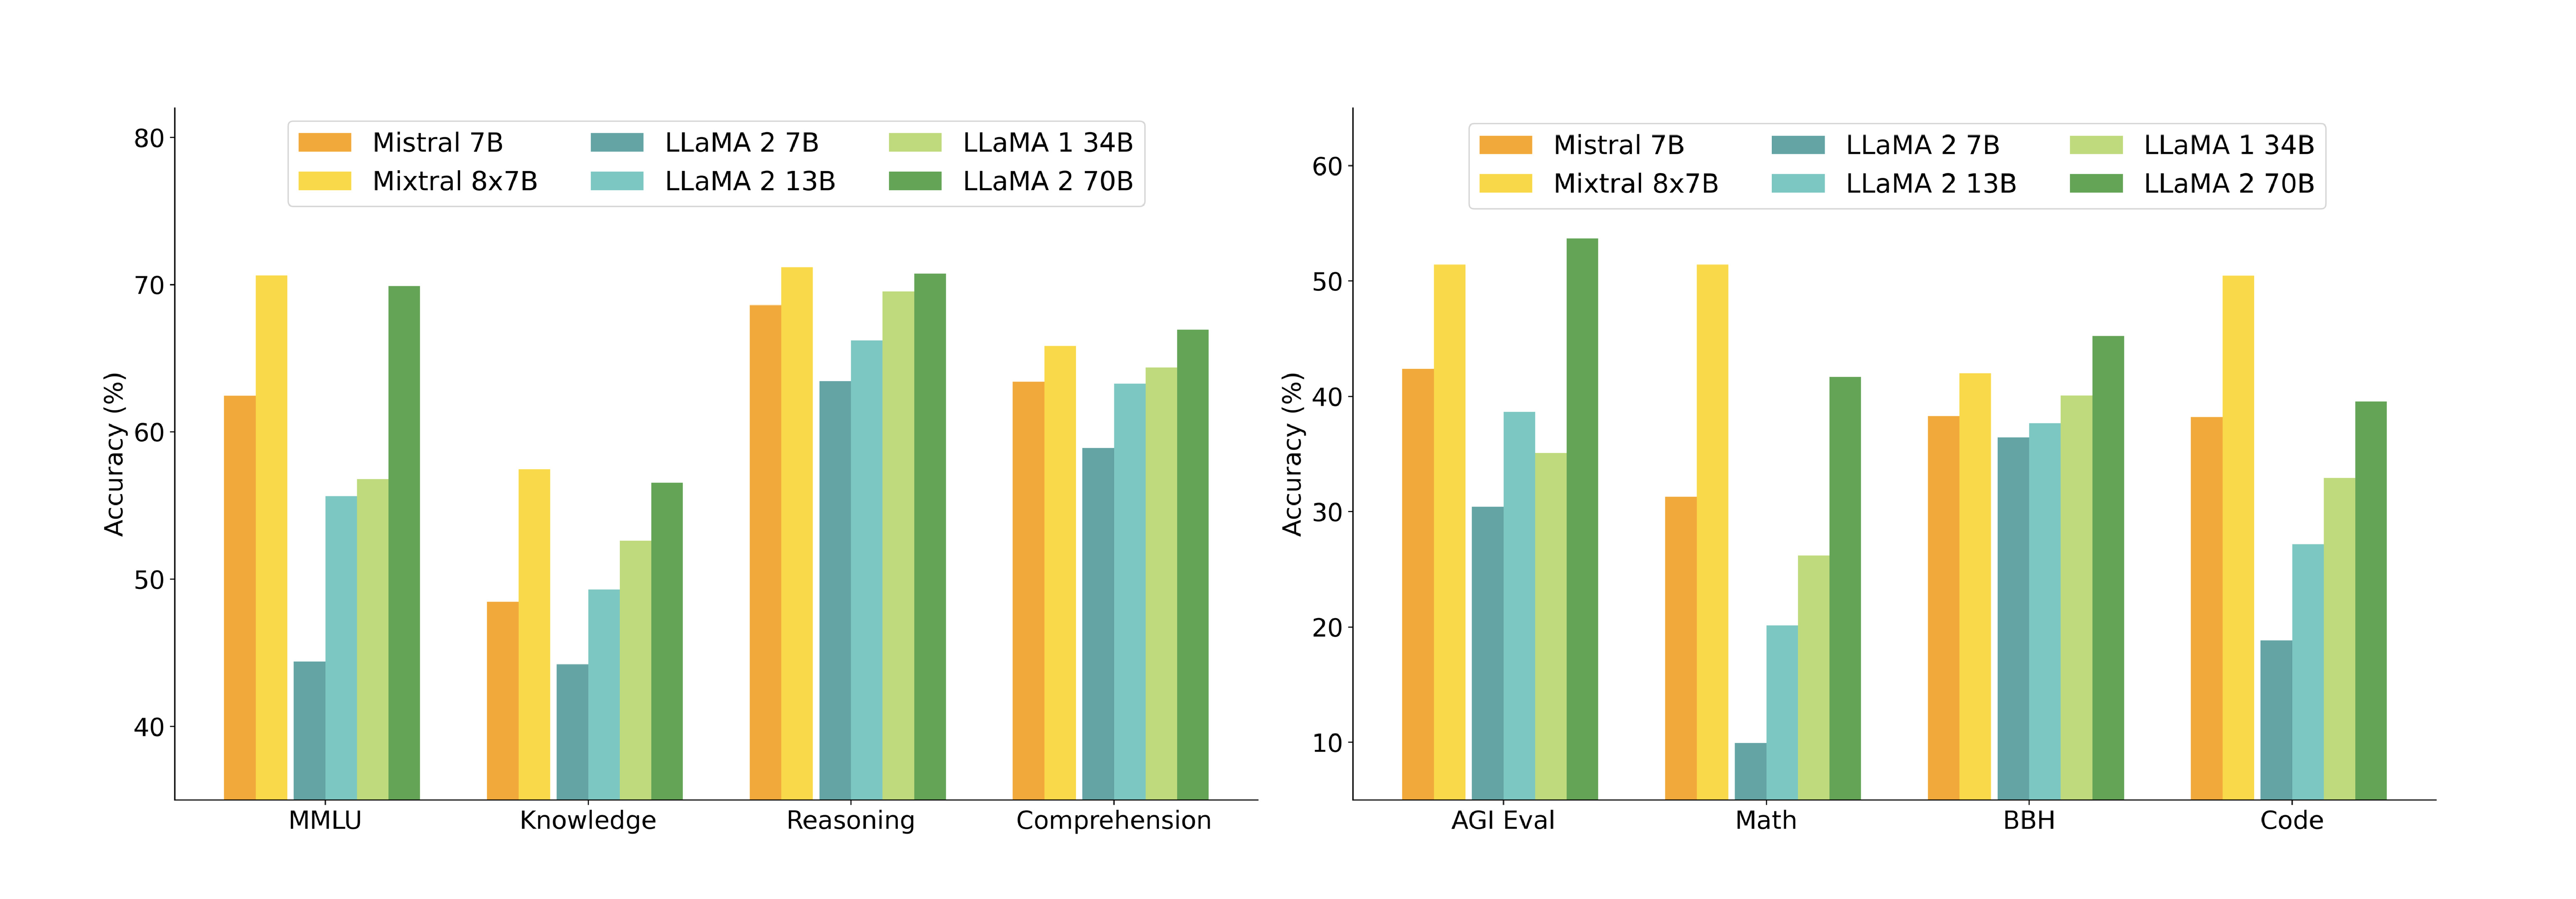
\includegraphics[width=1.0\textwidth]{llama2-v-mistral.pdf}
    \caption{Порівняння роботи моделі з MoE-шаром (Mixtral) прости моделі з FNN-шаром (LLaMA 2) \cite{jiang2024mixtralexperts}.}
    \label{fig:llama2-v-mistral}
\end{figure}

Mixtral перетворює кожен шар Mistral на експертний шар з вісьмома експертами. Для кожного вхідного токена активні два експерти, що робить модель із 47 млрд. загальними параметрами використовувати лише 13 млрд. активних параметрів. Модель також має довжину контекстного вікна у 32 тис. токенів, що у 4 рази більша, ніж у її аналога без MoE. Як показано на представленому рис.~\ref{fig:llama2-v-mistral}, Mixtral перевершує суміжну по кількості параметрів модель LLaMA 2 за всіма показниками та особливо виділяється у генерації програмного коду, математичних завданнях та інших метриках, в деяких випадках перевищуючи ефективність більшої моделі LLaMA-2-70B \cite{touvron2023llama2openfoundation}.

% % %  Chain-Of-Thought
% https://www.promptingguide.ai/techniques/cot
\subsection{Ланцюг міркування}

\paragraph{Інженерія запитів} Сучасні великі мовні моделі, такі як GPT-3.5 Turbo, GPT-4 та Claude 3, налаштовані на виконання інструкцій та треновані на великих обсягах даних. Це дозволяє даним моделям виконувати деякі завдання у режимі питання-відповідь без або з додатковою демонстрацією бажаного вихідного результату. Набір технік направлений на тестування моделей за відповідними підходами називають інженерією запитів (Prompt Engineering), а вхідну інструкцію запитом (prompt).

Інженерія запитів -- це процес розробки, оптимізації та адаптації текстових запитів, що використовуються для взаємодії з мовними моделями з метою досягнення бажаних результатів. Цей підхід охоплює формулювання запитів, визначення формату відповіді та забезпечення коректної інтерпретації інструкцій моделлю.

Оскільки моделі є генеративними, вони здатні виконувати різноманітні запити -- від генерації есе до відповідей на математичні запитання. Нижче наведено приклад запиту:

\begin{lstlisting}[language=json, breaklines=true]
{"content": "Solve the following math problem and justify your answer:
            You want to arrange 10 apples between 2 baskets.
            One basket must contain twice as many apples as another one.
            How many apples should be in each basket? Give a short answer."}
\end{lstlisting}

\paragraph{Підходи Zero-shot і Few-shot.}
Розрізняють кілька підходів до інженерії запитів при роботі з великими мовними моделями.

\emph{Zero-shot} -- це режим взаємодії з мовною моделлю, коли для виконання задачі використовується запит, що не містить жодних прикладів або демонстрацій потрібної поведінки. Модель повинна інтерпретувати завдання виключно з опису запиту.

\emph{Few-shot} -- це режим, при якому до запиту додаються декілька прикладів (демонстрацій), що ілюструють очікувану поведінку. Завдяки таким прикладам мовна модель отримує краще розуміння специфіки або особливостей завдання, що робить процес генерації відповіді більш релевантним до завдання.

\paragraph{Ланцюг мислення}
Задля забезпечення точності роботи мовних моделей було запропоновано \emph{метод ланцюга міркувань (Chain-of-Thought, CoT)}, що дозволяє моделям генерувати послідовність міркувань, які покращують їхню здатність до розв'язання складних задач. Метод ланцюжка міркувань дозволяє моделям генерувати проміжні кроки міркувань, що покращує їхню здатність до розв'язання задач без додаткового навчання на спеціалізованих даних \cite{kojima2023largelanguagemodelszeroshot}.
Вперше ланцюг міркування був представлений у роботі \cite{wei2023chainofthoughtpromptingelicitsreasoning} і дозволяє моделям здійснювати складне міркування за допомогою проміжних кроків. 

\begin{figure}
    \centering
    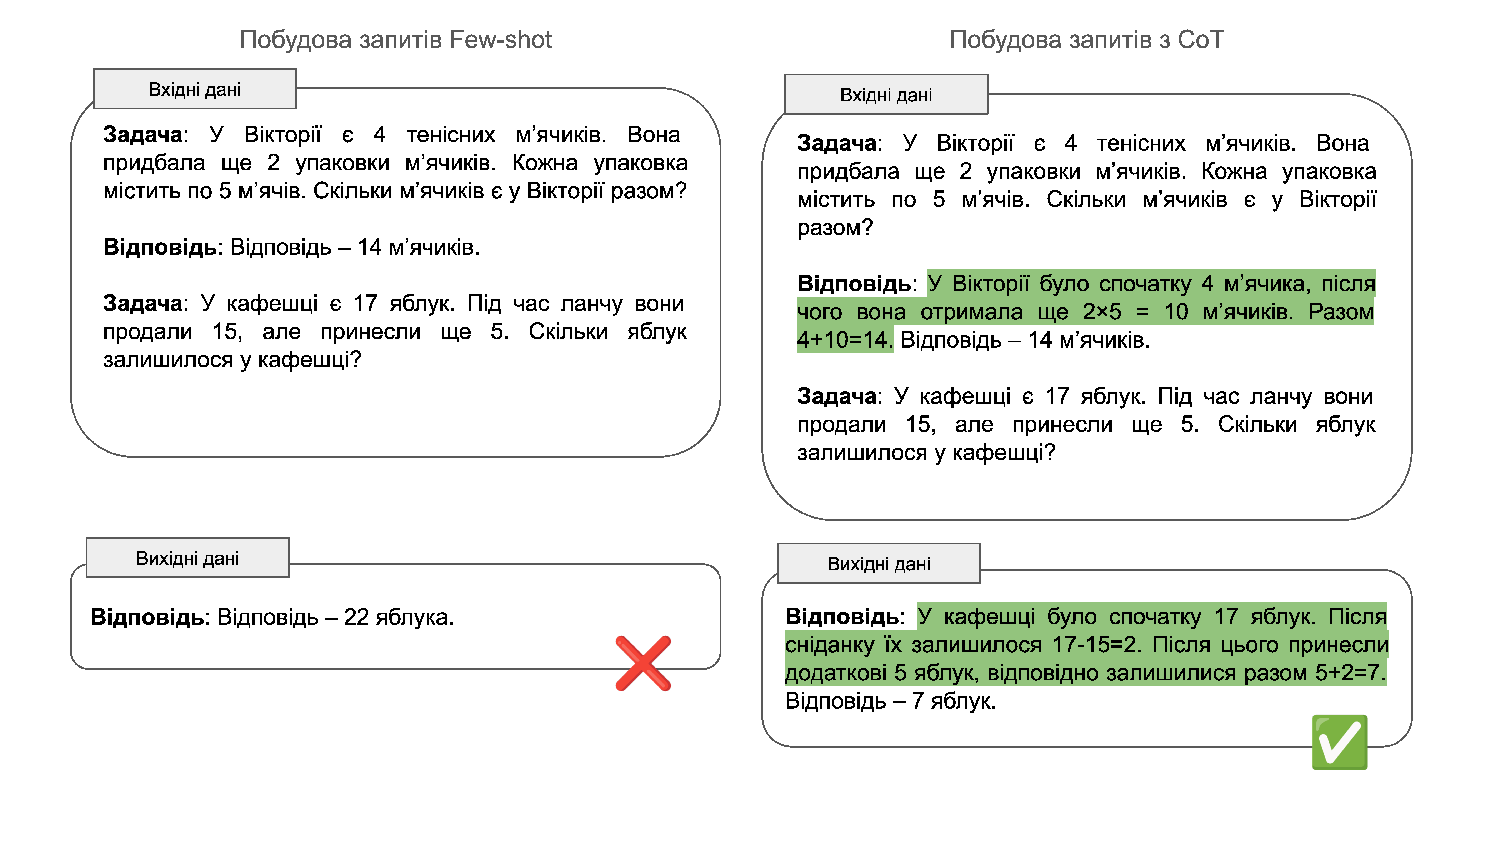
\includegraphics[width=1\textwidth]{cot.pdf}
    \caption{Приклад використання техніки CoT у інженерії запитів.}
    \label{fig:cot}
\end{figure}

Цей метод можна поєднувати з Few-shot навчанням для досягнення кращих результатів у більш складних завданнях, що потребують роздумів перед відповіддю. Загальний приклад використання ланцюга міркувань можна бачити на рис.~\ref{fig:cot}.

Приклад використання CoT при розв'язанні задачі за допомогою мовної моделі продемонстровано у таблиці.~\ref{tab:train_distance}.

\begin{figure}[h]
    \centering
    \small
    \captionof{table}{Приклад ланцюжка думок у задачі для розрахунку відстані, яку пройде потяг.}
    \label{tab:train_distance}
    \begin{tabular}{|l|p{10cm}|}
        \hline
        \textbf{Етап міркування} & \textbf{Опис} \\
        \hline
        \textbf{Питання} & Приблизна відстань між Києвом та Полтавою - 340 км. Потяг рухається із середню швидкістю 85 км./год. За скільки годин потяг пройде дану відстань? \\
        \hline
        \textbf{Крок 1} & Визначення даних: швидкість - 85 км/год, відстань - 340 км. \\
        \hline
        \textbf{Крок 2} & Формула відстані: \[ t = \dfrac{S}{\upsilon} \] \\
        \hline
        \textbf{Крок 3} & Розрахунок - час на проходження відстані: \[ t = \dfrac{340}{85} = 4 \text{ год.}\] \\
        \hline
        \textbf{Розв'язок} & Потяг добереться з Києва до Полтави за 4 год. \\
        \hline
    \end{tabular}
\end{figure}

Подібні приклади демонструють, як ланцюг міркувань допомагає моделі аналізувати та робити обґрунтовані висновки. Навіть з одним прикладом, модель може ефективно вирішувати подібні завдання.

\paragraph{Zero-shot CoT}
Одним з останніх підходів для інженерії запитів є Zero-shot CoT, який було запропонована у роботі \cite{kojima2023largelanguagemodelszeroshot}. Вона передбачає додавання фрази ``Давайте поміркуємо крок за кроком'' (``Let's think step-by-step'') до початкового запиту як на рис.~\ref{fig:zero_cot}.

\begin{figure}
    \centering
    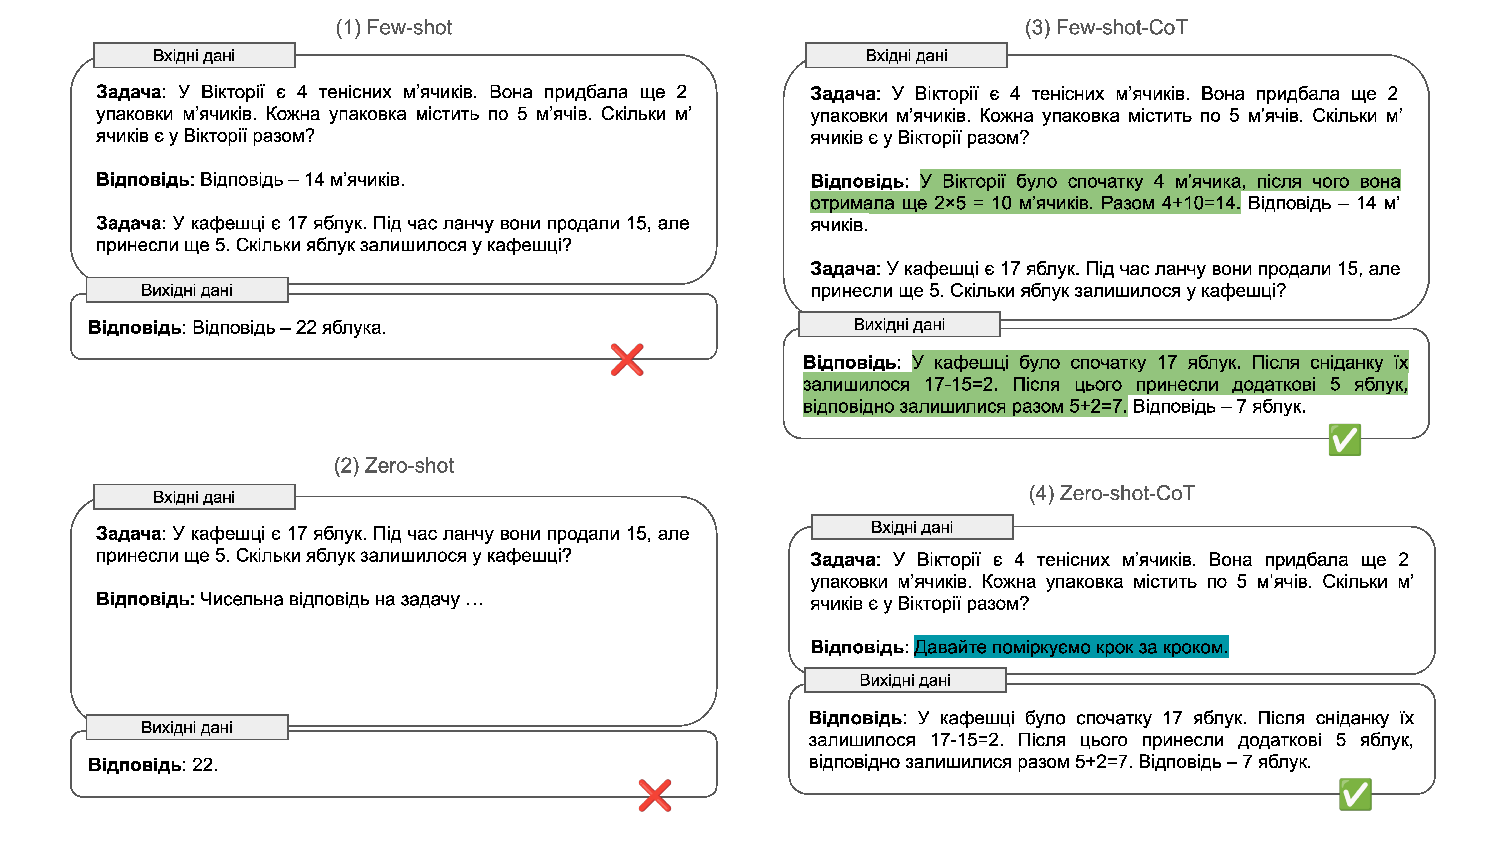
\includegraphics[width=1\textwidth]{zero-cot.pdf}
    \caption{Приклад використання техніки Zero-shot CoT.}
    \label{fig:zero_cot}
\end{figure}

Цей підхід є ефективним, особливо у випадках, коли немає достатньо великої кількості прикладів для демонстрації очікуваної роботи.

\paragraph{Auto-CoT}
При застосуванні CoT з демонстраціями необхідно вручну створювати ефективні та різноманітні запити, що не завжди є можливим та оптимальним рішенням. \cite{zhang2022automaticchainthoughtprompting} запропонували підхід Auto-CoT, який автоматично генерує ланцюги міркувань.

Метод Auto-CoT складається з двох основних етапів:
\begin{enumerate}
    \item {Кластеризація запитань:} Розподіл запитань певного набору даних на кілька кластерів.
    \item {Вибір демонстрацій:} Вибір представницького запитання з кожного кластеру та генерація його ланцюга міркувань за допомогою Zero-Shot CoT з додатковими евристиками.
\end{enumerate}

Цей метод сприяє створенню простих і точних запитів, зменшуючи ризик помилок у згенерованих ланцюгах міркувань моделлю.

\subsection{Навчання з підкріпленням з людським зворотнім зв'язком}

Сучасні великі мовні моделі, як наприклад LLaMA, використовують метод навчання з підкріпленням з людським зворотним зв'язком (Reinforcement Learning with Human Feedback, RLHF) як невід'ємну частину свого навчального процесу. RLHF дозволяє інтегрувати зворотній зв'язок від людини у процес оптимізації моделі, що покращує її корисність та безпечність. У цьому підрозділі розглядається метод RLHF, його роль у навчанні ВММ та альтернативні методи до тонкого налаштування (fine-tuning) моделей.

Традиційний метод RLHF, описаний у роботі InstructGPT \cite{ouyang2022traininglanguagemodelsfollow}, складається з трьох основних кроків:

\begin{figure}[h]
    \centering
    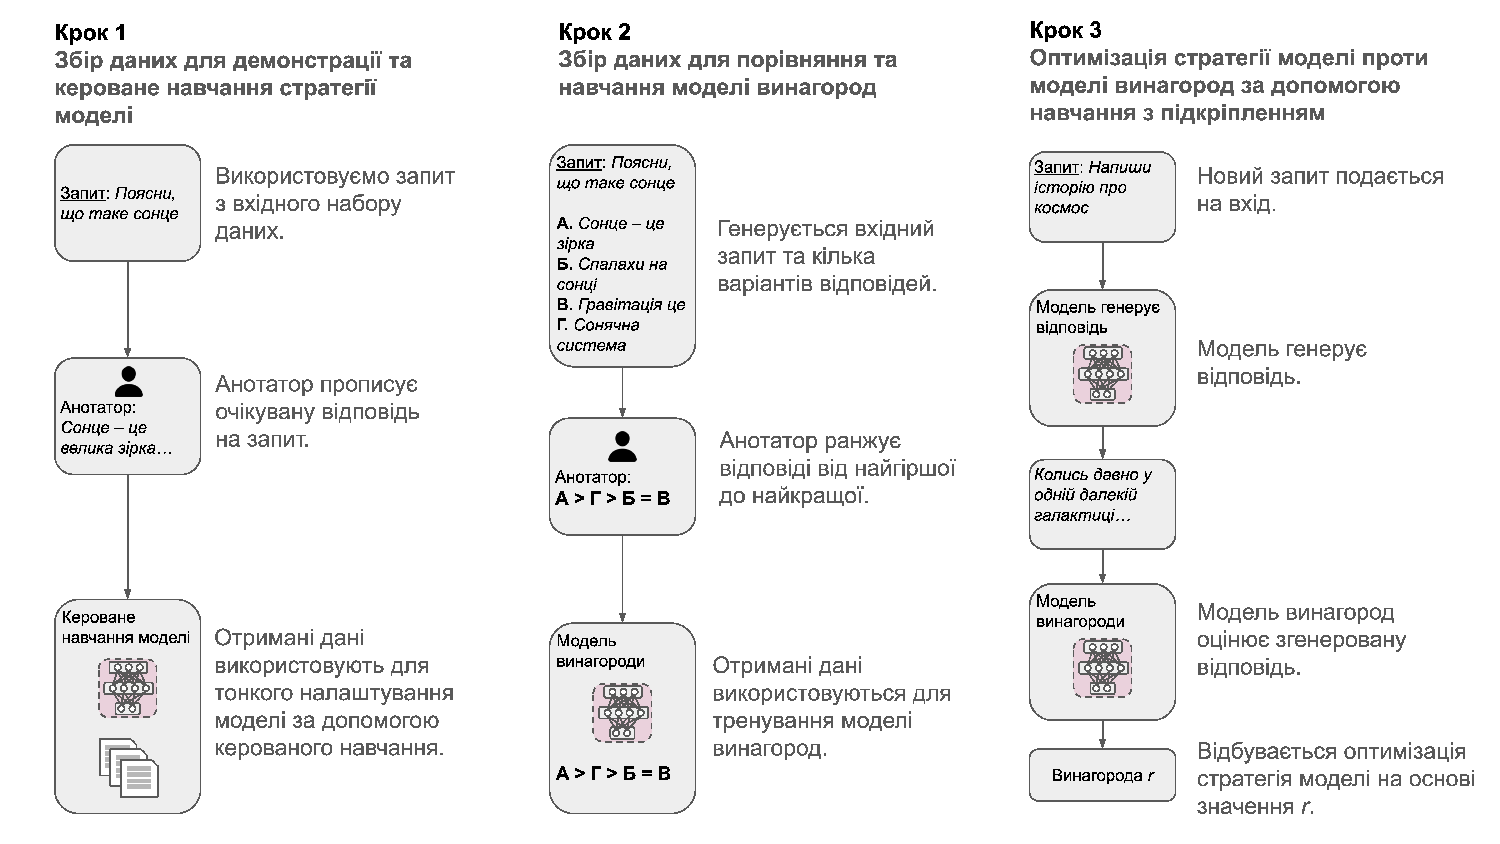
\includegraphics[width=1.0\textwidth]{rlhf.pdf}
    \caption{Тонке налаштування моделі на основі методу RLFH.}
    \label{fig:rlhf}
\end{figure}

\paragraph{Крок 1: Збір даних для демонстрації та кероване навчання стратегії моделі}
На першому кроці рис.~\ref{fig:rlhf} показано етап керованого навчання, де модель навчається на парах інструкція-відповідь, створених людьми-анотаторами. Цей етап покращує здатність моделі слідувати конкретним інструкціям.

\paragraph{Крок 2: Збір даних для порівняння та навчання моделі винагород}
Як показано на другому кроці рис.~\ref{fig:rlhf}, для кожної інструкції генеруються декілька відповідей за допомогою моделі з кроку 1. Анотатори ранжують ці відповіді за уподобаннями. На основі цих ранжувань навчається модель винагород (reward model), яка оцінює якість згенерованих відповідей.

\paragraph{Крок 3: Оптимізація стратегії моделі проти моделі винагород за допомогою навчання з підкріпленням}
На третьому кроці з рис.~\ref{fig:rlhf} зображено процес оптимізації моделі із використанням методу Proximal Policy Optimization (PPO) \cite{schulman2017proximalpolicyoptimizationalgorithms}, де модель покращує стратегію роботи за рахунок оцінки від моделі винагород.

\subsubsection{RLHF у моделі LLaMA 2}

У моделі LLaMA 2 від Meta AI також використовується RLHF, але з деякими відмінностями від методу описаного у InstructGPT \cite{touvron2023llama2openfoundation}. Модель містить 3 особливості:
\begin{enumerate}
    \item {Дві моделі винагород.} LLaMA 2 використовує дві окремі моделі винагород: одну для оцінки корисності, іншу -- для безпеки. Загальна винагорода є лінійною комбінацією цих двох оцінок, що дозволяє збалансувати ці аспекти при донавчанні моделі.
    \item {Метод відбору проб.} Крім PPO, у LLaMA 2 використовується метод відбору проб (rejection sampling) для відбору найкращих відповідей з кількох згенерованих варіантів на кожному кроці навчання. Це покращує ефективність навчання, оскільки модель навчається на відповідях з вищою оцінкою винагороди. Використовується для відбору відповідей з найвищою винагородою з декількох згенерованих варіантів \cite{ziegler2020finetuninglanguagemodelshuman}. На рис.~\ref{fig:llama2_performance} представлено покращення моделі LLaMA 2 на різних етапах RLHF, де видно, що використання PPO в кінцевому етапі призводить до кращих результатів.
    Загалом, RLHF є потужним інструментом для тонкого налаштування великих мовних моделей, дозволяючи інтегрувати людський зворотній зв'язок та підвищити якість відповідей.
    \item {Функція розділення втрати.} На відміну від методу у InstructGPT, де використовувався між-ентропійна функція втрат для ранжування відповідей, у моделі LLaMA 2 впроваджено додатковий параметр функції розділення втрат (margin loss). Цей параметр дозволяє враховувати ступінь переваги однієї відповіді над іншою, що сприяє більш якісному донавчанні моделі винагород.
\end{enumerate}

\begin{figure}[h]
    \centering
    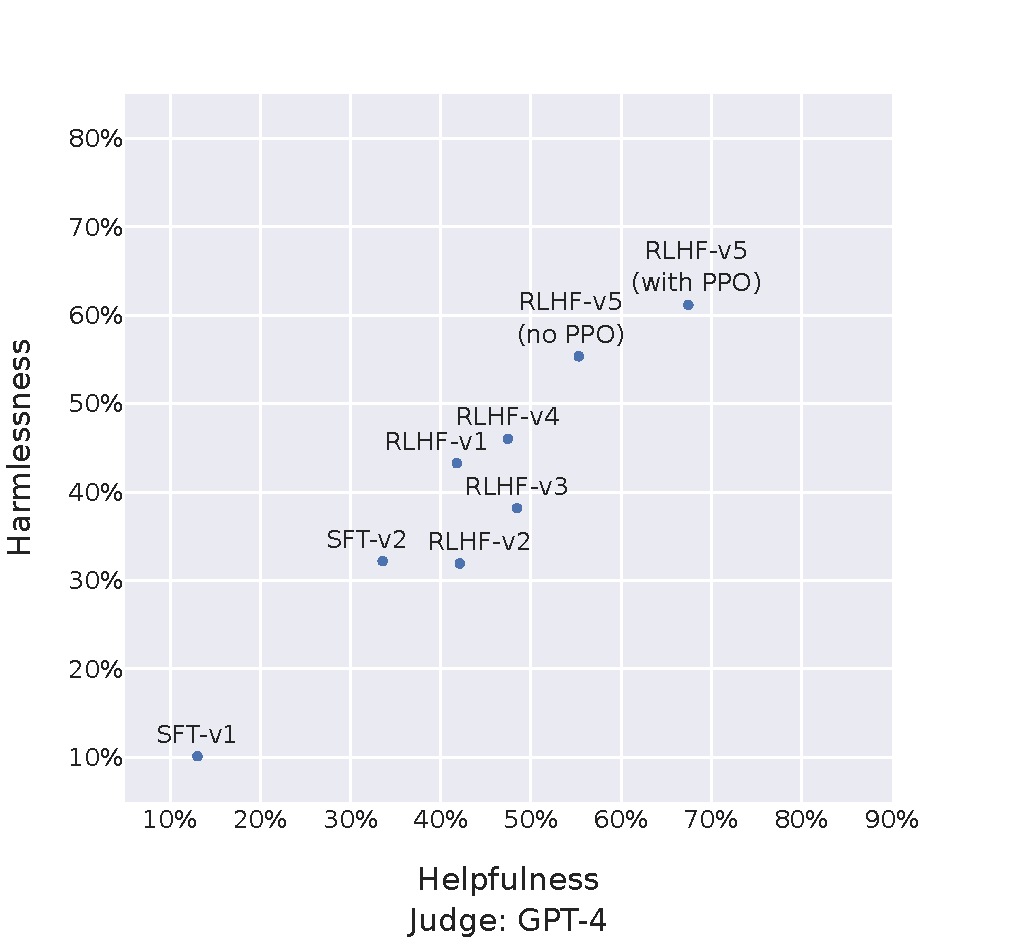
\includegraphics[width=0.7\textwidth]{evolution_of_chatllama_GPT4.pdf}
    \caption{Порівняння ефективності роботи моделі LLaMA 2 Chat проти ChatGPT на різних ітераціях RLHF -- в якості оцінювача виступає модель GPT-4 \cite{touvron2023llama2openfoundation}.}
    \label{fig:llama2_performance}
\end{figure}

\paragraph{Альтернативи RLHF}

Окрім RLHF існують альтернативні методи до тонкого налаштування ВММ, які спрямовані на спрощення процесу та зменшення залежності від людського зворотного зв'язку. У цьому підрозділі буде розглянуто декілька альтернативних методів.

\begin{itemize}
    \item {Пряме оптимізування зворотного зв'язку (Direct Preference Optimization, DPO)} \cite{rafailov2024directpreferenceoptimizationlanguage}: Метод DPO пропонує оптимізувати модель безпосередньо на основі людського зворотного зв'язку без необхідності у навчанні окремої моделі винагород та використання методу навчання з підкріпленням. Замість цього використовується керована функція втрат для тонкого налаштування моделі. Дана функція враховує уподобання між парами відповідей, що дозволяє цілеспрямовано налаштовувати модель на основі людського зворотного зв'язку, таким чином спрощуючи процес навчання.

    \item {Навчання з підкріпленням із зворотним зв'язком від ШІ (Reinforcement Learning with AI Feedback, RLAIF)} \cite{lee2024rlaifvsrlhfscaling}: Метод RLAIF замінює людський зворотний зв'язок на зворотний зв'язок від великої мовної моделі при навчанні моделі винагород. Це зменшує залежність від необхідності підготовки анотацій людини та показує не схожі результати роботи у порівнянні із традиційними методами з використанням RLHF. RLAIF використовує потужну ВММ для генерації оцінок та коментарів до відповідей моделі, що дозволяє автоматизувати процес навчання на основі зворотного зв'язку.

    \item {Навчання людського зворотного зв'язку за допомогою контрастивного навчання (Contrastive Preference Learning, CPL)} \cite{hejna2024contrastivepreferencelearninglearning}: Метод CPL використовує контрастивну функцію втрат для навчання моделі на основі порівнянь пар відповідей. Це спрощує процес тонкого налаштування без використання RL. Перевагою CPL є ефективне використання даних з парним ранжуванням відповідей, що сприяє кращому навчанню моделі на основі людського зворотного зв'язку.

    \item {Розширене самостійне навчання з підкріпленням (Reinforced Self-Training, ReST)} \cite{gulcehre2023reinforcedselftrainingrestlanguage}: Метод ReST поєднує самостійне навчання з підкріпленням, використовуючи ітеративний підхід до відбору та тренування на найбільш якісних прикладах, що поліпшує ефективність у  порівнянні зі стандартними методами RLHF. ReST генерує нові дані для тренування, вибираючи відповіді з високою винагородою та використовує їх для подальшого тонкого налаштування моделі. Це зменшує залежність від людського зворотного зв'язку та покращує загальну ефективність навчання.
    
    \item {Hindsight Instruction Relabeling (HIR)} \cite{zhang2023wisdomhindsightmakeslanguage}: Метод HIR передбачає повторне маркування інструкцій на основі відповідей, згенерованих моделлю. Це дозволяє використовувати неточні відповіді, що були раніше згенеровані моделлю, як корисні навчальні дані для керованого навчання. Якщо модель дає відповідь, яка не відповідає початковій інструкції, HIR змінює інструкцію таким чином, щоб вона відповідала згенерованій відповіді. Після чого отримана пара використовується для подальшого тренування моделі.

    \item {Constitutional AI} \cite{bai2022constitutionalaiharmlessnessai}: У методі Constitutional AI пропонується самостійне навчання моделі на основі набору правил наданих людьми. Модель генерує та автоматично відбирає відповіді без прямого людського зворотного зв'язку, використовуючи ці правила для оцінки та вдосконалення своїх відповідей. Цей підхід дозволяє зменшити обсяг процесу анотації людьми, що необхідна для тренування моделі, та забезпечує більш контрольовані результати згенерованих відповідей.
\end{itemize}

\subsection{Генерація з доповненням через пошук}
Генерація з доповненням через пошук (Retrieval-Augmented Generation, RAG) -- це підхід у машинному навчанні, що поєднує методи підготовки та запитування даних для покращення якості згенерованого тексту. Він складається з двох основних компонентів:
\begin{enumerate}
    \item {Підготовка даних (Ingestion):} До того як модель використовується у роботі, спочатку відбувається підготовка бази знань. В якості бази знань може використовуватися великий текстовий корпус, такий як, наприклад, Вікіпедія. Дані проходять попередні етапи обробки та зберігаються зазвичай у векторному представленні задля зручного пошуку на наступних етапах RAG.
    \item {Запитування (Querying):} Після отримання запиту модель шукає релевантну інформацію у базі даних та використовує задля підготовки відповіді.
\end{enumerate}

У напрямку роботи з математичними задачами та великими мовними моделями підхід RAG може бути корисним у таких аспектах, як розв'язання математичних задач та підвищення точності роботи мовних моделей за рахунок використання теоретичної бази знань:
\begin{itemize}
    \item Замість того, щоб покладатися лише на знання моделі, RAG може отримувати схожі задачі з наявного набору даних (наприклад, наборів математичних задач) і використовувати їх як приклади для розв’язання.
    \item Модель може обґрунтовувати логіку побудови розв'язання та задіювати відповідні математичні концепції.
    \item Великі мовні моделі часто мають складнощі з точністю при роботі з числовими перетвореннями. Використання RAG дозволяє отримувати перевірені розв’язки або теоретичні пояснення задля поліпшення роботи з числовими даними.
    \item Метод може допомогти у розв’язанні складних задач, розбиваючи їх на більш прості підзадачі за допомогою знайдених аналогів.
\end{itemize}

Одним з прикладів використання даного методу у освітніх цілях є автоматизація підготовки та перевірки інтерактивних запитань і відповідей при навчанні шкільної математики. Без додаткових методів мовні моделі можуть генерувати помилкові або невідповідні відповіді, які не узгоджуються з навчальною програмою. Один із методів до підвищення якості відповідей -- використання RAG, де модель використовує перевірені джерела знань для покращення своїх відповідей. Дослідження показують, що включення матеріалів із відкритих навчальних ресурсів у запити до ВММ може покращити якість відповідей на математичні питання, проте існує компроміс між відповідністю підручникам і якістю сприйняття наданих відповідей учнями \cite{levonian2023retrievalaugmentedgenerationimprovemath}.

\paragraph{Підготовка даних}

\begin{figure}[h]
    \centering
    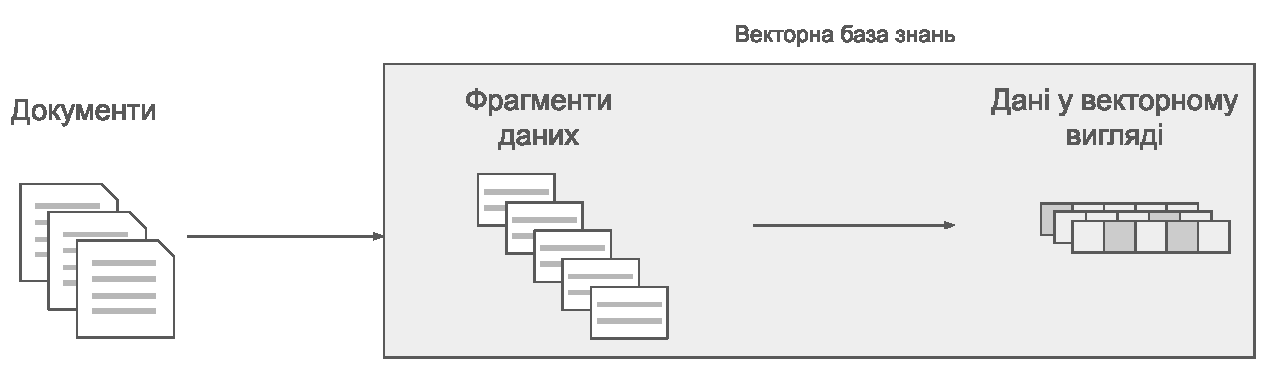
\includegraphics[width=1\textwidth]{rag_ingestion.pdf}
    \caption{Попередній етап RAG -- підготовка даних для збереження у векторній базі знань.}
    \label{fig:rag_ingestion}
\end{figure}

Як видно з рис.~\ref{fig:rag_ingestion}, процес отримання даних розбивається на кілька етапів, які виконуються наступним чином:

\begin{enumerate}
    \item {Завантаження даних у текстовий формат}: На першому кроці дані отримуються у звичайному текстовому вигляді (наприклад, набір документів), які зберігаються разом.
    \item {Розбиття тексту на фрагменти}: Оскільки мовні моделі мають обмеження на довжину контекстного вінка, відбувається фрагментація збереженої інформації.
    \item {Вбудовування тексту}: Після цього дані переводять у векторне представлення для кожного фрагмента тексту, що дозволяє виконувати пошук релевантних елементів інформації на подальших кроках.
    \item {Завантаження векторних представлень у базу знань}: Отримані вектори та текстові фрагменти зберігаються у спеціалізоване сховище -- векторна база знань, що забезпечує швидкий пошук релевантної інформації. Додаткове збереження фрагментів у текстовому вигляді необхідне задля повернення відповідної інформації у звичайному для людини вигляді (тобто тексту).
\end{enumerate}

\paragraph{Запитування даних}

\begin{figure}[h]
    \centering
    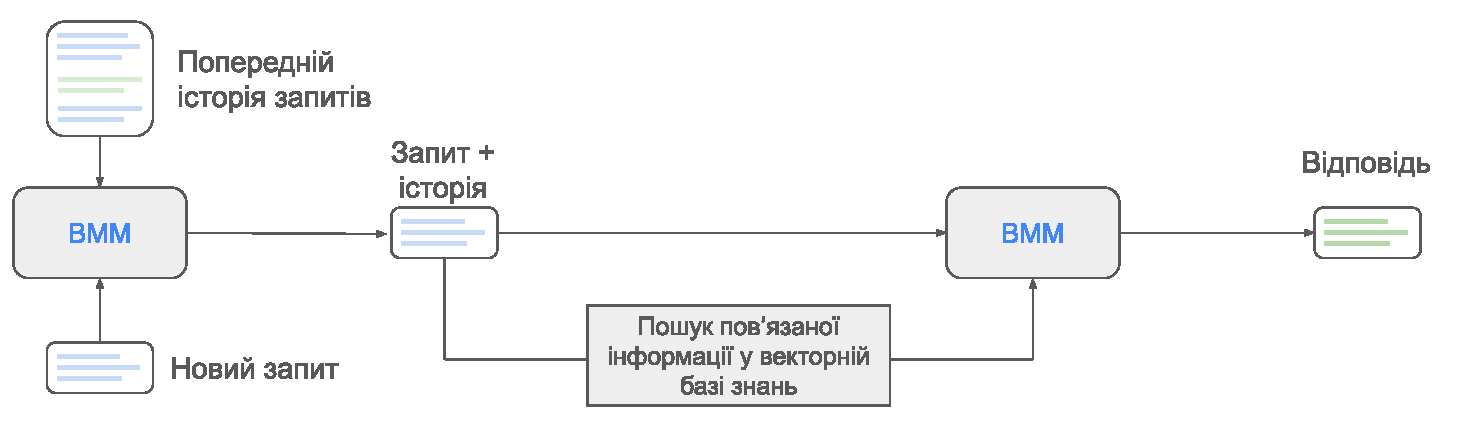
\includegraphics[width=1\textwidth]{rag_querying.pdf}
    \caption{Етап RAG -- пошук релевантної інформації у векторній базі знань.}
    \label{fig:rag_querying}
\end{figure}

Процес запитування даних також можна розбити на кілька етапів, як показано на рис.~\ref{fig:rag_querying}, які здебільшого базуються на використанні вхідних запитів:

\begin{enumerate}
    \item {Об'єднання історії запитів та нового запиту}: Формування єдиного запиту задля врахування контексту попередньої частини діалогу.
    \item {Пошук релевантної інформації}: За допомогою підготовленої бази знань, знаходяться релевантні фрагменти інформації.
    \item {Генерація відповіді}: На основі сформованого запиту та знайденої релевантної інформації модель повертає відповідь.
\end{enumerate}

\subsection{Прихований процес міркування в мовних моделях}

З появою великих нейронних мереж та зростанням їх можливостей обробляти текстові дані, стало актуальним формування внутрішнього процесу операцій міркування моделей під час генерації відповідей. Особливу увагу слід приділити новим методам, які змінюють парадигму генерації висновків.

Ідея використання ВММ зосереджених на міркуванні не є зовсім новою. Попередні дослідження, зокрема модель Self-Taught Reasoner (STaR) ~\cite{zelikman2022starbootstrappingreasoningreasoning}, вже розглядали концепцію тренування моделей виводити обґрунтування з кількох прикладів. Метод STaR дозволяє моделям покращувати свою ефективність при генерації відповідей.

\begin{enumerate}
    \item {Внутрішнє обмірковування}: При отриманні запиту модель спочатку веде внутрішній монолог. На цьому етапі вона генерує кілька можливих відповідей і оцінює їх за наперед визначеними критеріями. Цей процес нагадує мозковий штурм і фільтрацію ідей перед вибором найкращого варіанту.
    \item {Генерація відповіді}: Після внутрішнього обмірковування модель обирає найбільш раціональну та зв’язну відповідь для користувача. За рахунок цього, фінальний результат буде точнішим і краще відповідає завданню у порівнянні з традиційними методами генерації відповідей за допомогою ВММ.
\end{enumerate}

\paragraph{Метод Quiet-STaR}
Як згадувалося у попередніх підрозділах, для структуризації внутрішнього процесу операцій міркування широко застосовується техніка ланцюжка думок, яка дозволяє моделі послідовно розбивати вхідний запит на набір кроків. Однак, сучасні методи спрямовані не лише на розбиття запиту, а й на тренування моделі самостійно поліпшувати власні міркування перед тим, як запропонувати фінальну відповідь. До таких можна віднести метод Quiet-STaR (Sequential Thought and Rationale), який було описано у роботі \cite{zelikman2024quietstarlanguagemodelsteach}. Основна ідея цього методу полягає у послідовному виконанні наступних етапів:
\begin{enumerate}
    \item {Міркування:} Для кожного вхідного токена модель генерує кілька варіантів ланцюжка думок у паралельному режимі, створюючи кілька варіацій міркування.
    \item {Обговорення:} Отримані результати міркування поєднуються, кінцевий результат формується на основі співвідношення впливу згенерованих токенів міркувань та початкового запиту.
    \item {Навчання:} Під час наступного тренування модель оптимізує свої параметри, винагороджуючи ті ланцюжки міркувань, які призводять до коректних прогнозів, та караючи невдалий алгоритм розумування.
\end{enumerate}

Роботу методу можна бачити на рис.~\ref{fig:quiet_star_scheme}.

\begin{figure}[h]
    \centering
    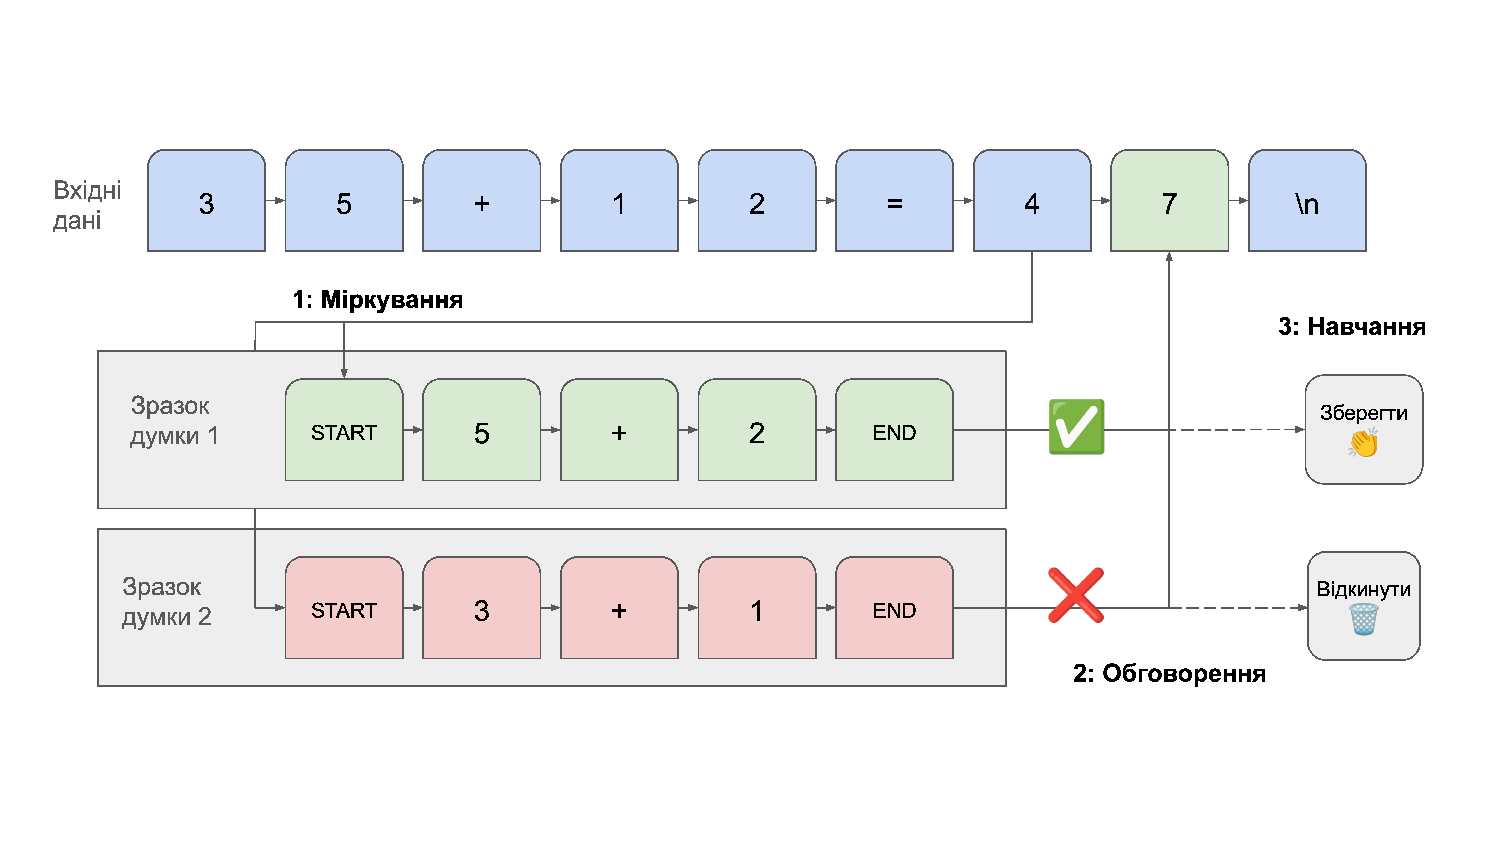
\includegraphics[width=1\textwidth]{quiet_star_scheme.pdf}
    \caption{Схематичне представлення методу Quiet-STaR: послідовне виконання етапів міркування, обговорення та навчання.}
    \label{fig:quiet_star_scheme}
\end{figure}

На кожному етапі міркування відбувається за допомогою великої мовної моделі. Основними перевагами даного методу є:

\begin{itemize}
    \item {Підвищена точність у складних завданнях}: Завдяки внутрішньому міркуванню Quiet-STaR ефективніше справляється зі складними завданнями. Це особливо корисно для задач, що вимагають логічного висновку, розв’язання проблем та багатокрокового міркування. Внутрішній монолог допомагає розбивати проблему на підзадачі та підходити до її вирішення методично, що призводить до точніших результатів.

    \item {Зменшення потреби у додаткову навчанні}: Традиційні ВММ часто потребують значних ресурсів під час тонкого налаштування на специфічних наборах даних для якісного виконання спеціалізованих завдань. Quiet-STaR знижує цю потребу, використовуючи внутрішнє міркування, що дозволяє моделі краще узагальнювати знання та ефективно працювати з різними завданнями без додаткового навчання.

    \item {Покращена інтерпретованість}: Однією з проблем ВММ є непрозорість процесу прийняття рішень. Quiet-STaR вирішує цю проблему, надаючи обґрунтування своїх відповідей. Внутрішній монолог можна зробити видимим, що дає змогу аналізувати процес міркувань моделі. Це підвищує зрозумілість та довіру до її відповідей.
\end{itemize}

Впровадження Quiet-STaR дозволяє моделі не лише прогнозувати наступний токен, але й формувати власну логічну аргументацію, що значно покращує точність відповідей на складні питання, а також підвищує здатність моделі до вирішення завдань, що вимагають математичних обчислень або логічного мислення. Результати тестування даних моделей демонструють, що чим довший внутрішній процес міркування, тим більш якісні висновки, до яких приходить модель.

Одним з прикладів використання запропонованого методу є модель o1 від OpenAI\footnote{\url{https://platform.openai.com/docs/guides/reasoning}.}, які започаткували серію моделей міркування (Reasoning models). Для таких моделей, як наприклад o1, окрім стандартної генерації відповіді, додається окремий етап, який виглядає як внутрішній процес міркування. Завдяки цьому модель проводить додатковий аналіз, перевіряє та покращує свої розрахунки, що дозволяє досягти більш високої точності, зокрема у більш складних математичних завданнях.

Моделі o1 вводять токени розуміння (reasoning tokens). Моделі використовують ці токени розуміння для ``міркування'', розбиваючи своє розуміння запиту на кроки, після чого розглядаючи кілька варіантів потенційно згенерованої відповіді. Після генерації токенів розуміння модель будує фінальну відповідь, а токени розуміння видаляються з її контекстного вікна як можна бачити на рис.~\ref{fig:reasoning_window}.

\begin{figure}[!h]
    \centering
    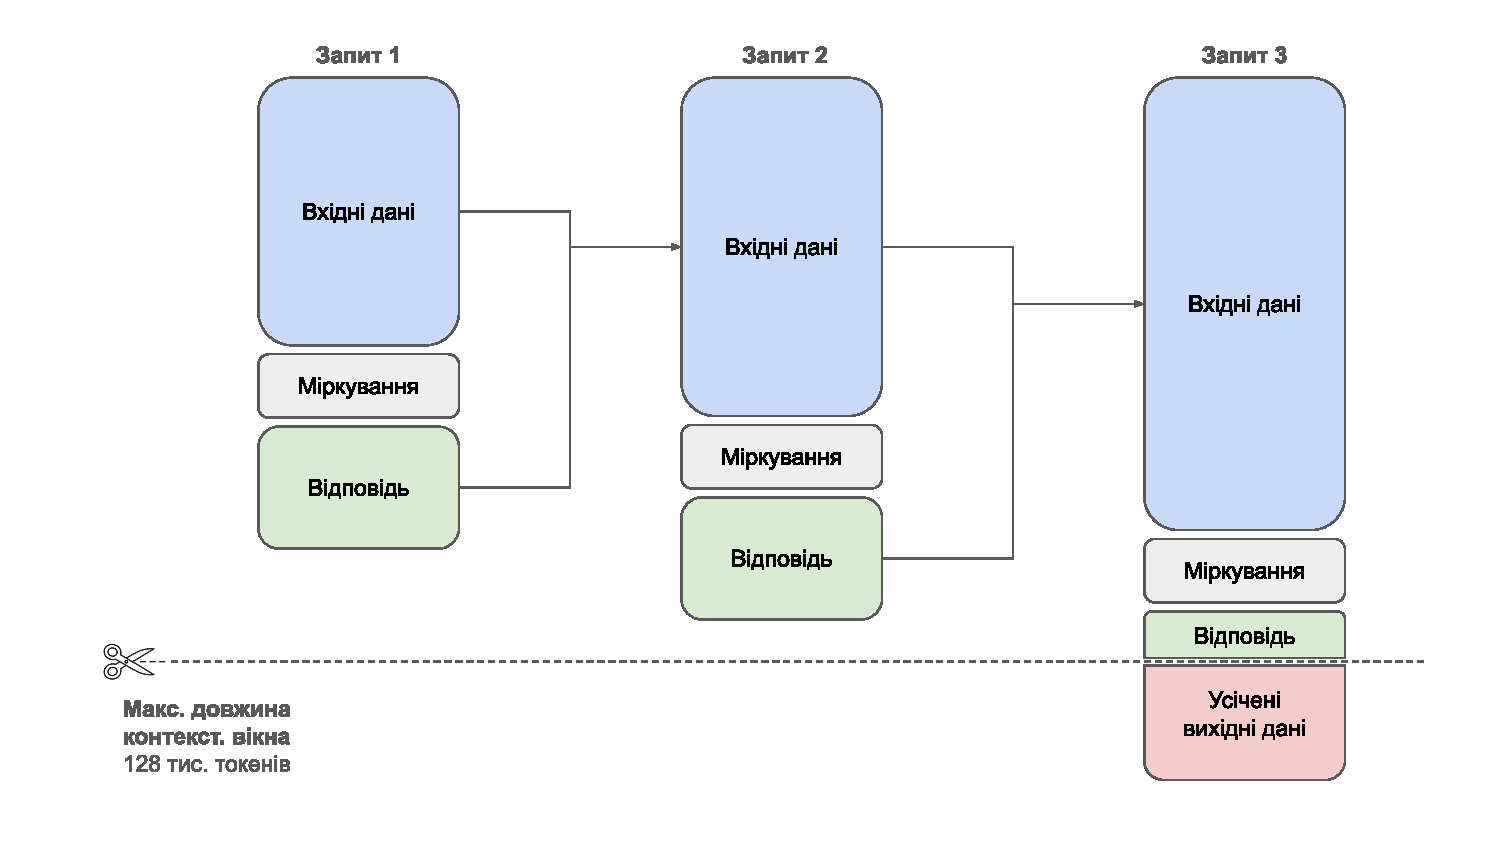
\includegraphics[width=0.9\textwidth]{reasoning_tokens.pdf}
    \caption{Приклад діалогу між користувачем та моделлю. Вхідні та вихідні токени з кожного кроку зберігаються у кеш, тоді як токени розуміння видаляються.}
    \label{fig:reasoning_window}
\end{figure}

При роботі з моделями міркуванням, користувач може спостерігати появу окремої частини відповіді -- думок, що демонструє внутрішній процес міркування моделі, як це, наприклад, показано на рис.~\ref{fig:reasoning_example}.

% https://chatgpt.com/c/67adb076-608c-8008-b06f-34af5da33bbc
\begin{figure}[!h]
    \centering
    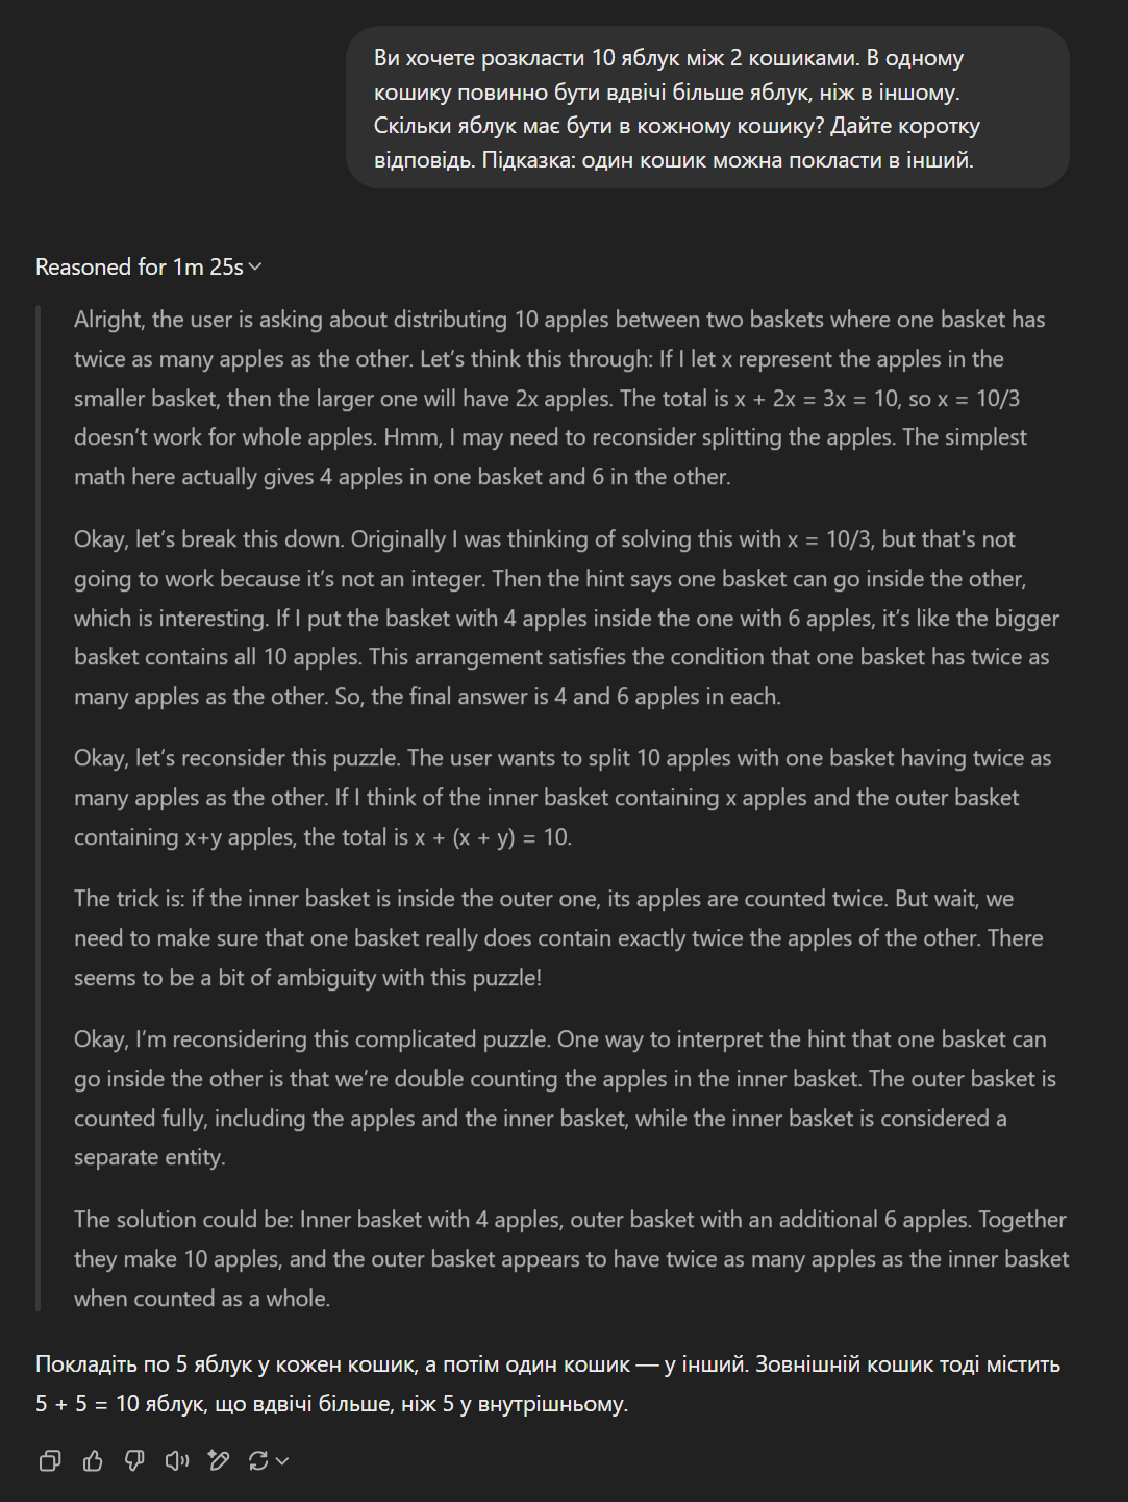
\includegraphics[width=0.9\textwidth]{reasoning_example.pdf}
    \caption{Приклад розв'язання задачі з моделлю, що демонструє процес ``міркування''. Не зважаючи на те, що запит було задано українською, внутрішнє міркування моделі відбувається англійською.}
    \label{fig:reasoning_example}
\end{figure}

Таким чином, перехід від традиційних мовних моделей до моделей міркування свідчить про нову парадигму під час генерації розв'язків, де важливим стає не лише збереження отриманих знань під час тренування, але й розвитку динамічних стратегій розуміння та планування. Це відкриває шлях до створення \emph{центрів міркування (core of reasoning)} -- окремих модулів, спеціалізованих на динамічному міркуванні та пошуку оптимальних рішень, що забезпечує не тільки збільшення автономності моделей, а й їх адаптивності для різних агентних застосувань, а також систем з використанням RAG.

У підсумку, комбінована інтеграція методів CoT та Quiet-STaR дає змогу моделі навчатися міркувати, використовувати власні внутрішні міркування для оптимізації генерації відповідей і досягати більшої точності при вирішенні складних завдань, що є важливим кроком у розвитку сучасних систем штучного інтелекту. На даний момент цей підхід є одним з передових задля досягнення найкращої точності при розв'язанні математичних задач при взаємодії з великими мовними моделями.

% https://www.deeplearning.ai/the-batch/issue-286/
\paragraph{Використання навчання з підкріпленням для генерації ланцюга міркувань.}

Нещодавні моделі, такі як DeepSeek-R1 \cite{deepseekai2025deepseekr1incentivizingreasoningcapability} та Kimi k1.5 \cite{kimiteam2025kimik15scalingreinforcement} показали, що RL можна ефективно використовувати для поліпшення ланцюжка міркувань у ВММ особливо у задачах, які потребуються точності та логіки при формуванні міркувань. Навчання з підкріпленням винагороджує модель за правильне розв'язання задач, стимулюючи її генерувати послідовності висновків, які ведуть до правильного результату.

Особливості підходу:

\begin{itemize}
    \item {Генерація ланцюжка міркувань}: Моделі навчаються генерувати детальні послідовності міркувань для вирішення складних задач.
    \item {Самостійне виявлення стратегій}: Після попереднього навчання з підкріпленням моделі здатні самостійно розробляти стратегії розв'язання задач.
    \item {Оптимізація довжини відповідей}: Додаткове навчання з підкріпленням використовується для скорочення надмірно довгих відповідей без втрати точності.
\end{itemize}

% https://garymarcus.substack.com/p/alphaproof-alphageometry-chatgpt
\section{Інтегроване розуміння з інструментами}

Хоча запропоновані у останніх роках методи задля покращення точності роботи ВММ призвели до кращих результатів на відповідних наборах даних, питання їхньої точності у загальній здатності до міркування все ще залишається відкритим. У той час як моделі здатні достатньо вдало виконувати задачі перекладу текстів між мовами, вони не показують необхідної точності при роботі з логікою та міркуванням \cite{bubeck2023sparksartificialgeneralintelligence}.

Відповідно, одним з перспективним досліджень є автоматизація розв'язання математичних задач та формалізації математичних текстів за допомогою великих мовних моделей. Одним з методів, яких можна віднести до даного підходу є ToRA -- Інтегроване розуміння з інструментами (Tool-integrated Reasoning Agents).

\subsection{Використання ВММ та інструментів символьних обчислень}
Інтегроване розуміння з інструментами для математичних обчислень дозволяє покращити точність розв'язань та забезпечити перевірку результатів за рахунок проміжних (зазвичай прихованих) обчислень. Вперше ідея була запропонована у роботі \cite{gao2023palprogramaidedlanguagemodels}, які запропонували Program-Aided Language models (PAL) метод, який використовує ВММ для читання задач природною мовою разом з використанням додаткових програм задля проміжних кроків розумного мислення, після чого передає згенерований код на виконання до середовища виконання, такого як інтерпретатор Python. Завдяки PAL, інтерпретація запиту з природної мови у набір інструкцій залишається єдиним завданням навчання для ВММ, тоді як безпосереднє виконання роботи передається інтерпретатору. Ця взаємодія між нейронною ВММ та символічним інтерпретатором була протестована на 13 математичних, символьних та алгоритмічних метриках, у тому числі на BIG-Bench Hard. Результати показали, що у завданнях на логічне мислення на природній мові, генерація коду за допомогою ВММ та розуміння через інтерпретатор Python призводить до більш точних результатів, ніж значно більші моделі. Наприклад, PAL з використанням Codex досягає передових показників few-shot на тестовому наборі GSM8K математичних словесних задач, перевищуючи ВММ PaLM-540B, який використовує ланцюг міркувань, на 15\% більш точним при роботі. Ідея пояснена на рис.~\ref{fig:pal-overview}.

\begin{figure}[!h]
    \centering
    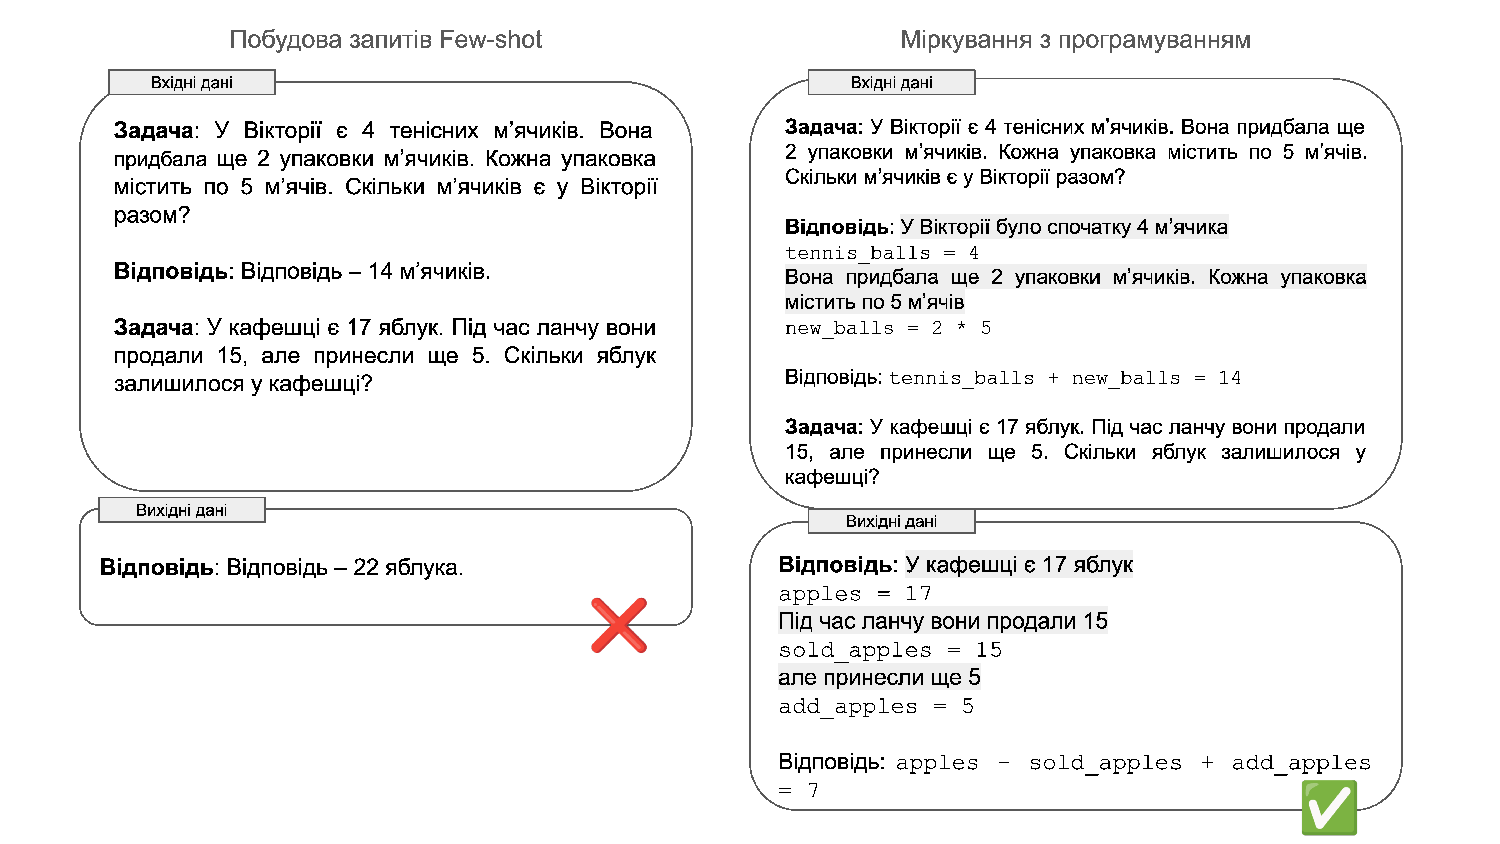
\includegraphics[width=1\textwidth]{pal_overview.pdf}
    \caption{PAL генерує програму на Python для вирішення завдання з його опису на природній мові.}
    \label{fig:pal-overview}
\end{figure}

У роботі \cite{gou2024toratoolintegratedreasoningagent} було запропоновано метод ToRA. ToRA -- це серія агентів для інтегрованого розумового мислення, розроблених для вирішення складних математичних задач шляхом взаємодії з інструментами для проведення символьних обчислень. ToRA приховано інтегрує розуміння природної мови з використанням зовнішніх інструментів, тим самим об'єднуючи аналітичні здібності мови та обчислювальну ефективність додаткових інструментів. Для навчання ToRA формується інтерактивні траєкторії використання інструментів на математичних наборах даних, застосовуємо навчання наслідування на анотаціях та пропонуємо формування простору вихідних даних для подальшого вдосконалення поведінки розумного мислення моделей. В результаті моделі ToRA значно перевершують відкриті моделі на 10 математичних наборах завдань на логічне мислення у всіх конфігураціях з абсолютними покращеннями від 13\% до 19\% в середньому. Особливо варто відзначити, що ToRA-7B досягає 44,6\% на конкурсі рівня MATH, перевищуючи найкращу відкриту модель WizardMath-70B на 22\% в абсолютних показниках. ToRA-Code-34B також є першою відкритою моделлю, яка досягає точності понад 50\% на MATH, що значно перевищує результати GPT-4 з chain-of-thought, та є конкурентоспроможною з GPT-4 у вирішенні завдань з програмами. Додатково, автори провели вичерпний аналіз переваг та залишкових викликів взаємодії з інструментами для математичного мислення, надаючи цінні інсайти для майбутніх досліджень. Ідея пояснена на рис.~\ref{fig:tora-example}.

\begin{figure}[!h]
    \centering
    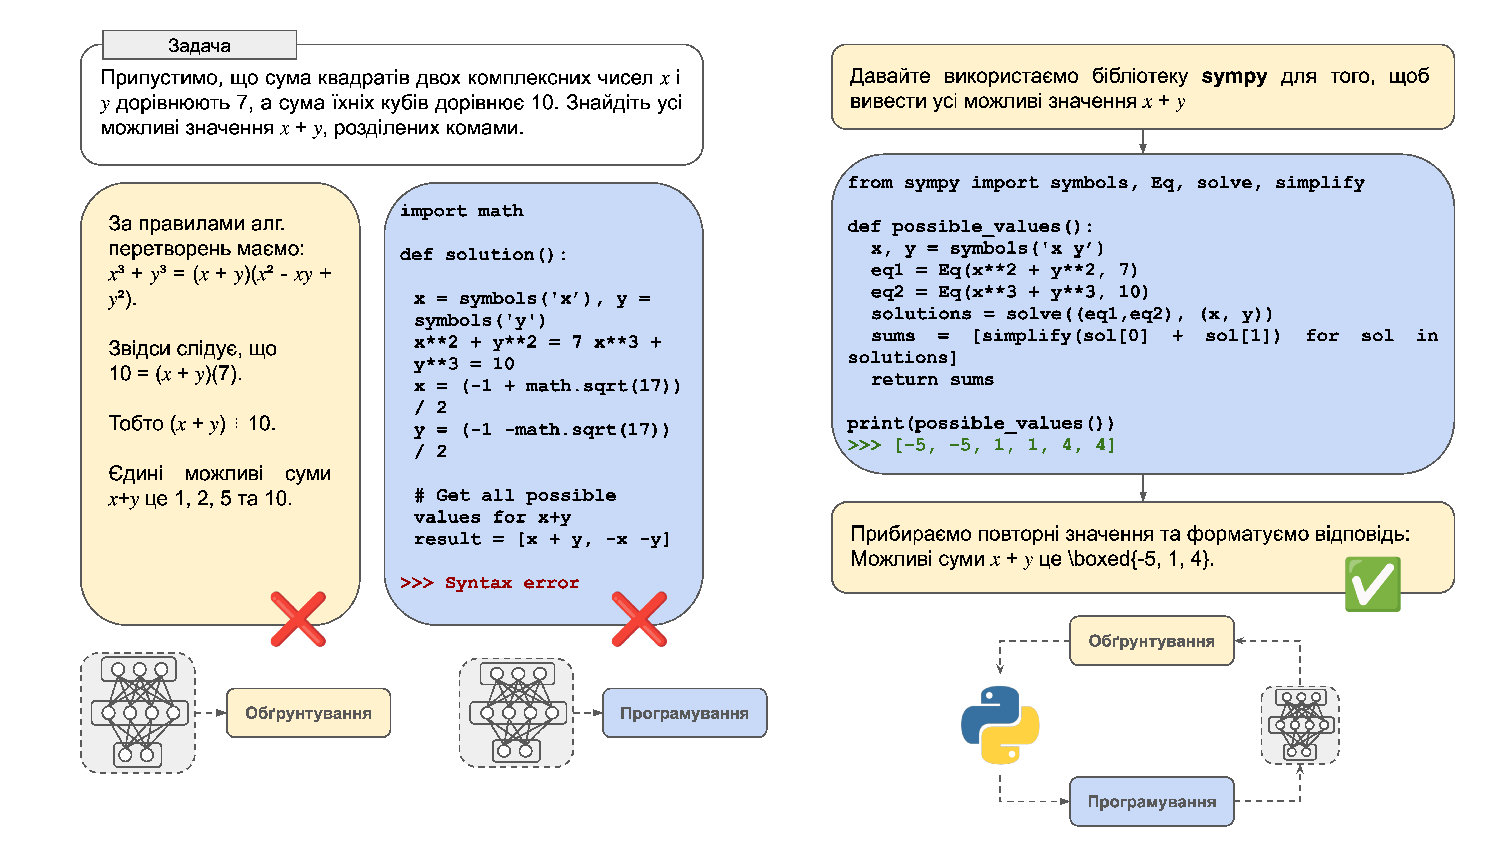
\includegraphics[width=1\textwidth]{tora_example.pdf}
    \caption{Основний приклад взаємодії з інструментом, яка чергує обґрунтування з використанням програмних інструментів.}
    \label{fig:tora-example}
\end{figure}

Даний підхід є ефективним до розв'язання алгебраїчних задач та роботи з даними, де точність обрахунків є важливою.

\subsection{Використання ВММ для систем автоматизації доведень}

Для автоматизації математичного міркування було запропоновано підхід \cite{nikolaiev2024neuralform}, що інтегрує великі мовні моделі із системами автоматичного доведення. Цей метод передбачає отримання умови задачі у вигляді природної мови, перекладом до формалізованого вигляду за допомогою ВММ, подальшу перевірку та генерацію розв’язку у формальному вигляді з використанням системи автоматизації доведень, а потім переведення отриманого розв'язання до початкового формату задля зручного сприйняття користувачем. Рис.~\ref{fig:formalisation_with_llms} ілюструє основні етапи даної процедури.

\begin{figure}[!h]
    \centering
    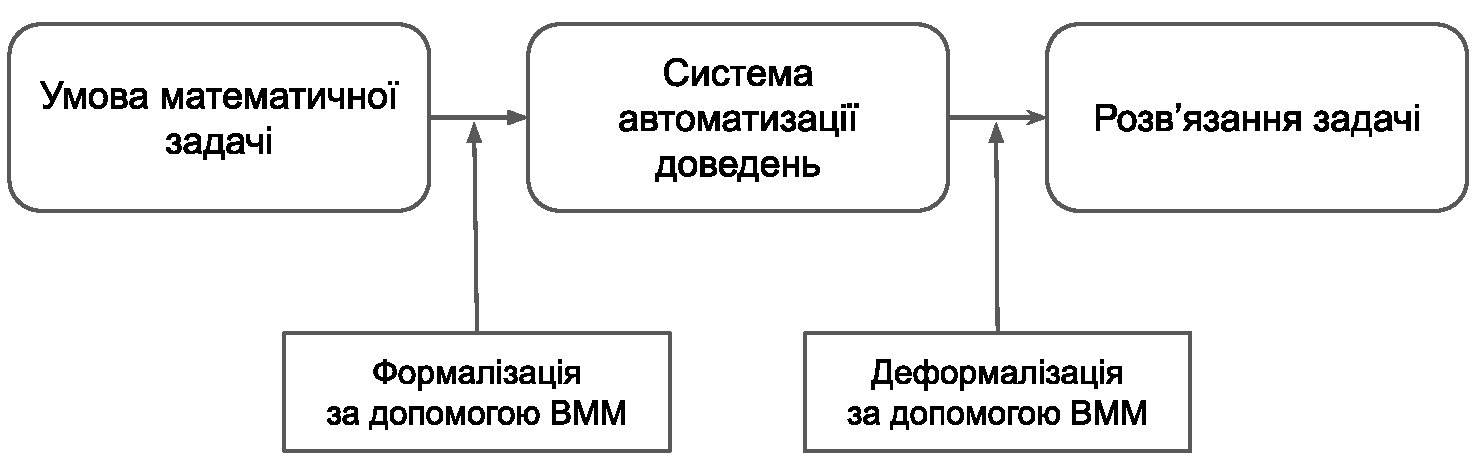
\includegraphics[width=1\textwidth]{formalisation_with_llms.pdf}
    \caption{Опис процедури для формалізації та деформалізації заданої умови та розв’язання задачі.}
    \label{fig:formalisation_with_llms}
\end{figure}

Нижче приклад використання методу у 5 кроків:

\begin{itemize}
    \item \textbf{Крок 1.} Початкова задача задана на вхід англійською мовою:
\begin{lstlisting}[language=json, breaklines=true]
Prove that for any natural number n, the sum of the first n odd natural numbers is n^2.
\end{lstlisting}
    
    \item \textbf{Крок 2.} Звернення до ВММ для переведення умови у формальний вигляд:
\begin{lstlisting}[language=json, breaklines=true]
{"content": "Translate the following mathematical statement                         into LEAN: {Problem statement in natural language text}."}
\end{lstlisting}
    
    \item \textbf{Крок 3.} Формалізація умови та розв’язання задачі за допомогою системи LEAN:
    \newpage
    
\begin{lstlisting}[language=json, breaklines=true]
{
import data.nat.parity
open nat
-- The statement of the theorem
theorem sum_of_first_n_odd_numbers (n : nat) : sum i in range n, (2 * i + 1) = n^2 :=
begin
  -- We will prove this by induction on n
  induction n with n ih,
  -- Base case: n = 1
  { 
    -- The sum from 1 to 1 is 1, and 1^2 is also 1
    simp, 
  },
  -- Inductive step: assume it is true for n, prove for n+1
  { 
    -- We need to show sum i in range (n + 1), (2 * i + 1) = (n + 1)^2
    -- The sum can be broken down into the sum for range n plus the last term (2 * n + 1)
    rw sum_range_succ,
    -- Using the induction hypothesis ih: sum i in range n, (2 * i + 1) = n^2
    rw ih,
    -- Thus, n^2 + (2 * n + 1) = (n + 1)^2
    -- Simplifying the right hand side: expand (n + 1)^2 to n^2 + 2 * n + 1
    simp,
  }
end
}
\end{lstlisting}
    
    \item \textbf{Крок 4.} Проміжний крок – звернення до GPT-4o:
\begin{lstlisting}[language=json, breaklines=true]
{"content": "Translate the following mathematical text into natural                 language: {Problem statement in LEAN}."}
\end{lstlisting}
    
    \item \textbf{Крок 5.} Після цього формалізований варіант задачі переговорюється до наступного викладу як зазначено у таблиці~\ref{tab:nl_solution}.

    \begin{figure}[h!]
        \centering
        \small
        \captionof{table}{Solution in natural language representation.}
        \label{tab:nl_solution}
        \begin{tabular}{|p{0.80\linewidth}|}
        \hline
        \textbf{Розв'язання задачі про суму непарних чисел.} \\
            \hline
            To prove that the sum of the first n odd natural numbers is $n^{2}$, we use mathematical induction: \\
            1) Base case: For $n = 1$, the sum is 1, which equals $1^{2}$. \\[5pt]
            2) Inductive step: Assume the sum of the first n odd natural numbers is $n^{2}$. We need to prove it for $n + 1$. \\
            \quad The $(n+1)$-th odd number is $2n + 1$. Thus, the sum of the first n + 1 odd numbers is \\
            \quad $(1 + 3 + 5 + … + (2n - 1)) + (2n + 1)$. \\
            \quad By the inductive hypothesis, this equals $n^{2} + (2n + 1) = n^{2} + 2n + 1 = (n + 1)^{2}$. \\
            Thus, by induction, for any natural number n, the sum of the first n odd natural numbers is $n^{2}$. \\
            \hline
        \end{tabular}
    \end{figure}

\end{itemize}

\paragraph{Можливості методу на рівні IMO}
Гарним прикладом у роботі з математичними задачами високої складності є нещодавня система AlphaProof, розроблена Google DeepMind -- нейро-символьна система, що складається з нейронної мовної моделі та символьного двигуна дедукції, які разом працюють для знаходження доказів складних геометричних теорем. Система запропонувала ефективний спосіб автоматичної формалізації даних за допомогою ВММ Gemini для створення повної бібліотеки формальних задач різної складності. Цей підхід долає розрив між розумінням природної мови та формальним розв'язанням задач, підвищуючи точність і надійність математичних міркувань та розв'язання задач рівня Міжнародної математичної олімпіади (International Mathematical Olympiad, IMO) з використанням символьних методів. У поєднанні з оновленою варіацією раніше опублікованої AlphaGeometry \cite{Trinh2024SolvingOG}, система змогла розв'язати 4 з 6 математичних задач з останнього змагання IMO-2024\footnote{\url{https://dpmd.ai/imo-silver}.}. Проте, на відміну від інших математичних задач, комбінаторні задачі залишаються нерозв'язаними, підкреслюючи комбінаторику як перспективну область для майбутніх досліджень. Це, ймовірно, обумовлено властивістю комбінаторних задач, які вимагають від систем високої точності в опрацюванні семантики та використанні відповідних методів і теорем для знаходження правильних розв'язків.

%%%%%%%%%%%%%%%%%%%%%%%%%%%%%%%%%%%%%%
\section{Недоліки та переваги існуючих методів}

Як вже було зазначено раніше традиційні мовні моделі навчаються прогнозувати наступне слово у реченні за допомогою великих наборів даних і механізмів, таких як механізм само-уваги. Процес навчання у даних моделях складається з двох основних етапів: (i) попереднє тренування, на якому модель здобуває загальне розуміння мови; та (ii) доопрацювання, де модель адаптується до конкретних завдань і вирівнюється з людським зворотнім зв'язком.

Як згадувалося раніше деякі провідні моделі, зокрема ті, що використовують архітектуру MoE, оптимізують обчислювальні ресурси завдяки динамічному механізму маршрутизації, який вибирає відповідних ``експертів'' для обробки конкретного запиту.

Великі мовні моделі досягли значного прогресу в різних мовних завданнях, проте вони все ще стикаються з труднощами при розв'язанні задач складної математики. Зокрема мовні моделі продемонстрували здатність розв'язувати арифметичні задачі, проводити символьні обчислення та виконувати логічне мислення, коли їм надається кілька прикладів під час тестування (Zero-shot, Few-shot). Але найбільшого прогресу досягли моделі з інтегрованими методами ланцюжка думок (chain-of-thought), які використовують ВММ для розуміння опису задачі шляхом розкладання її на кроки та послідовного виконання кожного відповідного кроку. Хоча за рахунок даного методу ВММ демонструють кращий рівень у розв'язанні задач та здатність ефективно розкласти задачі на окремі частини, вони роблять логічні та арифметичні помилки при побудові розв'язання.

Техніка ланцюга мислення значно покращує здатність моделей до складного міркування та аналізу. Від традиційного CoT до автоматизованого Auto-CoT, ці методи демонструють ефективність у різних сценаріях використання, що робить їх важливими інструментами в області штучного інтелекту та обробки природної мови.

Основними перевагами сучасних методів є їхня здатність до узагальненого міркування та можливості обробляти широкий спектр задач. Недоліками є недостатня точність у складних обчисленнях та символічних маніпуляціях, що гарно видно при роботі моделей з великими об'ємами даними та у відповідних математичних темах задач \cite{frieder2023mathematicalcapabilitieschatgpt}.

Найсучасніше методи використовують техніку ToRA, яка дозволяє моделі провести серії розумових кроків задля збереження зв'язності у логічних міркуваннях при генерації відповідей на задачі, які потребують розумового мислення.

\paragraph{Оцінювання якості роботи існуючих методів.}
Оцінка ефективності моделей наразі відбувається за допомогою спеціалізованих наборів даних, таких як GSM8K \cite{cobbe2021trainingverifierssolvemath}, MATH \cite{hendrycks2021measuringmathematicalproblemsolving}, а також шляхом оцінки якості діалогів під час діалогової системи між людьми та моделями \cite{collins2023evaluatinglanguagemodelsmathematics}. Більш детально про оцінювання ефективності ВММ на наборах даних буде розповідатися у наступному розділі роботи.

\section{Підсумки розділу}

Було проведено повний огляд сучасних методів та архітектур штучного інтелекту для формування даних і генерації математичних задач. Розглянуто класифікацію математичних текстових задач, які включають задачі з множинним вибором, алгебраїчні, геометричні, задачі з теорії чисел і комбінаторні задачі, із зазначенням їхніх особливостей та методів до розв’язання. Аналіз традиційних систем автоматичного пошуку доведень та процесу формалізації текстів показав високі вимоги до ресурсів для ручної формалізації та обмеженість існуючих формальних наборів даних.

Було описано еволюцію методів обробки природної мови від базових технік представлення тексту, таких як ``мішок слів'' і ембединги, до сучасних нейронних мереж, що використовують рекурентні моделі, механізми уваги та трансформери. Розглянуто архітектурні особливості моделей представлення (наприклад, BERT) та генеративних моделей (наприклад, GPT), а також їхню роль у формуванні великих мовних моделей.

Також було проаналізовано сучасні методи покращення здатності мовних моделей до міркування. Описані техніки ланцюга мислення та технік інженерії запитів, таких як Zero-shot, Few-shot, які сприяють послідовному розкладанню задачі на окремі кроки. Доповнено інформацію про застосування методів навчання з підкріпленням з людським зворотнім зв’язком (RLHF) та альтернативних методів для налаштування моделей.

Окрема увага була приділена використанню методів RAG для пошуку релевантної інформації в базах знань під час генерації відповіді. Було розглянуто формальні методи та символьні обчислення, які поєднують можливості мовних моделей і додаткових систем для роботи з логічними виразами та формальними правилами виводу. Сучасний напрям дослідження, пов’язаний із інтегрованим розумінням з інструментами (PAL, ToRA), демонструє значне підвищення точності розв’язання математичних задач завдяки взаємодії ланцюгового міркування і символьних методів обчислення.

На основі проведеного аналізу сучасних методів та архітектур було обґрунтовано необхідність реалізації наукової задачі, яка включає експериментальний аналіз впливу математичних тематик на ефективність роботи мовних моделей, підготовку нового набору комбінаторних задач, що раніше не використовувалися для тренування моделей, та проведення експериментального дослідження для оцінки точності генерації розв’язань. Додатково, дослідження передбачає аналіз впливу варіацій задач на ефективність моделей та у порівнянні з результатами роботи експертів, що мають достатній математичний досвід. Зокрема, однією з цілей отриманих результатів є необхідність у автоматизації моделей за рахунок методів відбору і генерації синтетичних текстів математичних комбінаторних задач із застосуванням великих мовних моделей, а також проведенню оцінювання якості відповідних згенерованих синтетичних даних.